% VMI Analysis GUI — user manual
%
% Build (from the repository root, twice for the table of contents):
%   pdflatex -output-directory=.cache/manual-build docs/manual.tex
%   pdflatex -output-directory=.cache/manual-build docs/manual.tex
%   copy .cache/manual-build/manual.pdf docs/manual.pdf
%
% Inline code is set with \code{...}; write \_ for underscores. Long tokens
% contain generated \allowbreak{} hints so that narrow table cells wrap instead
% of overflowing. They only affect line breaking and are harmless when a token
% is edited.
\documentclass[11pt,a4paper]{article}

\usepackage[T1]{fontenc}
\usepackage[utf8]{inputenc}
\usepackage{lmodern}
\usepackage[margin=2.0cm,headheight=14pt]{geometry}
\usepackage{microtype}
\usepackage{xcolor}
\usepackage{booktabs}
\usepackage{longtable}
\usepackage{array}
\usepackage{enumitem}
\usepackage{titlesec}
\usepackage{fancyhdr}
\usepackage{hyperref}
\usepackage{url}
\urlstyle{tt}
\usepackage{tikz}
\usepackage{graphicx}
\graphicspath{{docs/}{./}}
\usepackage{caption}
\usepackage{amsmath}
\usetikzlibrary{arrows.meta,positioning}

\definecolor{vmcoral}{HTML}{CC785C}
\definecolor{vmdark}{HTML}{181715}
\definecolor{vmcream}{HTML}{FAF9F5}
\definecolor{vmhairline}{HTML}{E6DFD8}

\hypersetup{
  colorlinks=true,
  linkcolor=vmcoral,
  urlcolor=vmcoral,
  pdftitle={VMI Analysis GUI — User Manual},
  pdfauthor={vmi-analysis-gui contributors},
  pdfsubject={Velocity-map imaging photoelectron analysis pipeline and web interface}
}

\titleformat{\section}{\Large\bfseries\color{vmdark}}{\thesection}{0.8em}{}
\titleformat{\subsection}{\large\bfseries\color{vmdark}}{\thesubsection}{0.6em}{}
\setlist{itemsep=1pt,topsep=3pt}
\usepackage{etoolbox}
\AtBeginEnvironment{longtable}{\scriptsize}
\setlength{\tabcolsep}{3pt}
\setlength{\emergencystretch}{2em}

\pagestyle{fancy}
\renewcommand{\sectionmark}[1]{\markboth{#1}{#1}}
\fancyhf{}
\fancyhead[L]{\small\color{vmcoral}VMI Analysis GUI}
\fancyhead[R]{\small\color{vmcoral}\rightmark}
\fancyfoot[C]{\small\thepage}
\renewcommand{\headrulewidth}{0.2pt}

\newcolumntype{L}[1]{>{\raggedright\arraybackslash}p{#1}}
\newcommand{\code}[1]{\texttt{#1}}
\newcommand{\file}[1]{\code{\small #1}}

\begin{document}
\sloppy

\begin{titlepage}
  \centering
  \vspace*{2.0cm}
  {\Huge\bfseries VMI Analysis GUI\par}
  \vspace{0.6cm}
  {\Large User Manual\par}
  \vspace{0.8cm}
  {\large Velocity-map imaging photoelectron analysis\\
   and the NiceGUI web interface\par}
  \vfill
  
\includegraphics[width=12cm]{logo.png}
  \vfill
  \begin{tabular}{ll}
    Application version & 0.1.0 \\
    Document revision & 1.0 \\
    Date & \today \\
    License & Apache License, Version 2.0 \\
  \end{tabular}
  \vfill
  {\small This manual describes the panels, input fields, processing
   stages, output files, and operating constraints of the application.
   Bundled CPBASEX uses the MIT License.}
\end{titlepage}

\markboth{Contents}{Contents}
\tableofcontents
\clearpage

\section{Introduction}
\label{sec:intro}

The application analyzes camera frames from velocity-map imaging (VMI)
experiments. It can produce detector images, calibrated energy spectra, and
angular anisotropy parameters ($\beta$). The repository provides:

\begin{itemize}
  \item a set of standalone Python command-line programs that perform the
        numerical analysis, and
  \item a NiceGUI web interface with panels for individual tools and an
        ordered Pipeline job.
\end{itemize}

Supply your experiment data through the interface or on the command line.
The Binning, PES, and Pipeline panels are immature and need restructuring.
Their sections document the current behavior.

\subsection{The analysis chain}
\label{sec:chain}

\begin{figure}[h]
\centering
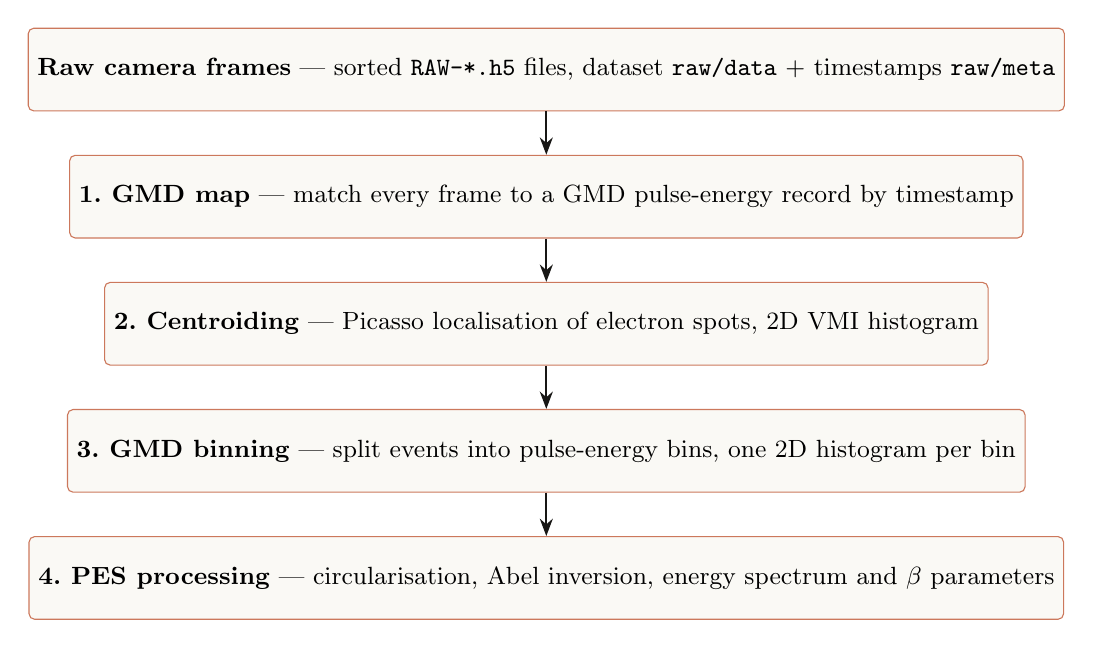
\begin{tikzpicture}[
  node distance=0.55cm,
  box/.style={draw=vmcoral, rounded corners=2pt, fill=vmcream,
              align=center, minimum width=9.4cm, minimum height=1.05cm,
              font=\small},
  arr/.style={-{Stealth[length=2.2mm]}, draw=vmdark, thick}]
  \node[box] (raw) {\textbf{Raw camera frames} — sorted \file{RAW-\allowbreak{}*.\allowbreak{}h5}
                    files, dataset \file{raw/\allowbreak{}data} + timestamps \file{raw/\allowbreak{}meta}};
  \node[box, below=of raw] (gmd) {\textbf{1.\ GMD map} — match every frame to a
                    GMD pulse-energy record by timestamp};
  \node[box, below=of gmd] (cen) {\textbf{2.\ Centroiding} — Picasso
                    localisation of electron spots, 2D VMI histogram};
  \node[box, below=of cen] (bin) {\textbf{3.\ GMD binning} — split events
                    into pulse-energy bins, one 2D histogram per bin};
  \node[box, below=of bin] (pes) {\textbf{4.\ PES processing} — circularisation,
                    Abel inversion, energy spectrum and $\beta$ parameters};
  \draw[arr] (raw) -- (gmd);
  \draw[arr] (gmd) -- (cen);
  \draw[arr] (cen) -- (bin);
  \draw[arr] (bin) -- (pes);
\end{tikzpicture}
\caption{The four-stage analysis pipeline. Stages 1--4 are available as
individual panels and as a single Pipeline run.}
\label{fig:chain}
\end{figure}

Run each stage from a terminal or from the web interface. The job panels
launch the command-line programs as subprocesses. Trig Calibration runs
interactive remapping and fitting in the web process.

\subsection{How this manual is organised}

Section~\ref{sec:install} explains installation, starting the interface, and
a first end-to-end run.
Section~\ref{sec:shared} describes behaviour shared by every panel: the
window layout, the Run/Stop control, the job queue, the log console, the file
picker, the image-inspection overlay, and saved settings. Then
Section~\ref{sec:data} describes the files the user must supply.
Section~\ref{sec:panels} is the reference: one subsection per panel, with
every field and button. Sections~\ref{sec:outputs} and~\ref{sec:calibration}
explain the files produced and the energy calibration procedure, and
Sections~\ref{sec:cli}--\ref{sec:trouble} cover command-line use and
troubleshooting. The appendices hold a glossary and the main formulas.

Conventions used in the field tables: \emph{verbatim} labels reproduce the
interface text exactly; ``saved key'' is the name under which the value is
persisted (Section~\ref{sec:settings}); ``CLI flag'' is the equivalent
command-line argument; ``default'' is the value shown on a fresh
installation, i.e.\ before any saved setting exists.

\section{Installation and first run}
\label{sec:install}

\subsection{Requirements}

\begin{itemize}
  \item Python 3.12 or newer and \code{uv}, the project manager used for
        installation and for launching the application.
  \item Optional: \code{ffmpeg} on the system path, needed only to write
        MP4 movies in the Movie panel (otherwise a GIF is written).
  \item Optional: MATLAB, needed only for the CPBASEX inversion backend in
        PES. The default PyAbel backend is pure Python.
\end{itemize}

\subsection{Install}

\begin{verbatim}
git clone <repository-url>
cd vmi-analysis-gui
uv sync
\end{verbatim}

\code{uv sync} creates the virtual environment and installs every
dependency, including the web interface. The package is installed in
editable mode, so later source edits take effect without reinstalling.

\subsection{Start the interface}

\begin{verbatim}
uv run vmi-analysis
\end{verbatim}

The application serves \code{http:/\allowbreak{}/\allowbreak{}localhost:13517} and opens a browser.
Set \code{VMI\_\allowbreak{}GUI\_\allowbreak{}PORT} to use another port and
\code{VMI\_\allowbreak{}GUI\_\allowbreak{}NO\_\allowbreak{}SHOW=1} to suppress the browser window. If the port is
busy, the program prints a suggested free port with ready-to-paste commands
and exits; it does not switch automatically.

Each analysis stage can also be run without the interface:
\code{uv run python -\allowbreak{}m vmi\_\allowbreak{}analysis.<module> -\allowbreak{}-\allowbreak{}help} lists the options of
every program (Section~\ref{sec:cli}).

\subsection{A first end-to-end run}

For a single-image distortion check, run Centroiding first.
Open its raw VMI image in Trig Calibration. Fit and accept rings.
Send the calibration to Circularize. Compare the two polar views after the run.

The following sequence uses the current Binning and PES panels.

\begin{enumerate}
  \item \textbf{GMD Map.} Choose the folder of \code{RAW-\allowbreak{}*.\allowbreak{}h5} files and the
        GMD timestamp file, choose an output map path, and Run. The result is
        a frame-to-GMD map.
  \item \textbf{Centroiding.} Choose the same HDF5 folder and an output
        directory. First tick \emph{Tuning mode only}, enter a tuning frame
        index or leave it blank for a random frame, and run to inspect
        detection. Adjust box size or minimum net gradient
        if spots are missed or noise dominates. Then untick it and run the
        full batch. Expect a checkpoint, a 2D histogram, and summary figures.
  \item \textbf{Binning.} Choose the checkpoint, the GMD map, the output
        directory, the threshold values, and the weighting mode. Run to
        produce one 2D histogram per GMD bin.
  \item \textbf{PES.} Put the two circularisation calibration files in
        \code{circularization/\allowbreak{}}, keep the PyAbel backend, and Run. The
        results are energy spectra, anisotropy parameters, and an archive of
        all arrays.
\end{enumerate}

To run the same stages in one job, open \emph{Pipeline}. Set the dataset,
GMD timestamp file, and map output. Click \emph{Run pipeline}. The job
runs stages 1--4 in order. With \emph{Skip stages whose outputs exist}
selected, the job checks for the declared output files before each stage.

\subsection{What to check after the first run}

\begin{itemize}
  \item The GMD map has two header lines plus one row per frame; the console
        reports the time-difference statistics and the share of frames within
        20 and 40\,ms.
  \item The Centroiding tuning figure shows localisations on real spots, and
        the final summary shows a VMI image with a physically plausible
        spectrum.
  \item Binning produced the expected number of \code{.\allowbreak{}npy} files
        (thresholds plus one) with the expected suffix for the chosen weight
        mode.
  \item PES produced three overview figures and a \code{.\allowbreak{}npz} archive.
        PES plots use energy channels with the current fixed alpha of 1.
        Centroiding has its own alpha field (Section~\ref{sec:calibration}).
\end{itemize}

\section{The shared interface}
\label{sec:shared}

All panels follow the same pattern: a section heading with a one-line
description, a cream feature card holding the parameter form, one
Run/Stop control, a dark log console, and a results area below it. This
section describes the parts that behave identically everywhere; the
panel-specific fields are in Section~\ref{sec:panels}.

\subsection{Window layout and tabs}
\label{sec:tabs}

Open \emph{Settings} to set the job limit or control shutdown after a
disconnect. Use the same menu to save and load workflow files.
The tabs appear in this order:
\code{GMD Map}, \emph{Movie}, \emph{Dark Frame}, \emph{Accumulate},
\code{Centroiding}, \emph{Binning}, \emph{Trig Calibration}, \emph{Circularize}, \emph{PES},
\code{Pipeline}.

Every panel is built when the page loads and keeps its own run state,
progress, log, and results. Switching tabs does not stop or restart work.

\subsection{The Run/Stop control}
\label{sec:runstop}

Each job panel uses one button to start or stop its job. Trig Calibration
uses separate controls for remapping, processing, and fitting. The job
button reads \emph{Run} when idle (\emph{Run pipeline} in Pipeline). It changes to

\begin{itemize}
  \item \emph{Stop} while the panel's job is running,
  \item \emph{Cancel queued} while it is waiting for a slot or for a file
        conflict to clear,
  \item a disabled \emph{Stopping\ldots} during cleanup.
\end{itemize}

Stopping a queued job removes it from the queue immediately. Stopping a
running job terminates the whole subprocess tree (on Windows with
\code{taskkill /\allowbreak{}T /\allowbreak{}F}), so the analysis program and its worker processes
end together. Stopping one panel's job never stops another panel's job.
The button never starts a second job from a stale click, and it returns to
\code{Run} when the job finishes, fails, or is cancelled.

A job that is active when the page is reloaded is reattached by its panel
from the job name, restoring its Run/Stop state, progress, and current log.
A job that had already finished before the reload is not restored.

\subsection{Job queue, concurrency and file reservations}
\label{sec:queue}

All job panels share one queue. Open \emph{Settings} to set
\emph{Maximum concurrent jobs}. Choose a value from 1 to 10. The default is 2.
Running jobs continue when you lower the limit. The server saves the value
for the next start.

The queue also enforces file safety. Each submitted command declares the
files and directories it reads and writes. A job whose output overlaps
another job's input or output waits, and shows a reason such as
\code{Waiting for <job>: <path>} or \emph{Waiting for a concurrent job
slot}. Unrelated jobs can start in the free slots. Only one job per panel
may be active at a time. Jobs launched by the Pipeline panel reserve the
inputs and outputs of all four stages for the whole run.
GMD Map can write a file inside a standalone Centroiding output directory
when the map path is separate from the run's inputs and outputs.

The MATLAB/CPBASEX backend takes an exclusive lock because the MATLAB script
uses a shared working file, so MATLAB jobs never overlap each other or a job
writing the same directory.

\subsection{The log console and progress}
\label{sec:log}

Every panel has a dark console under the form. It shows the exact command
that was launched, prefixed with \code{[gui] \$}, followed by the merged
standard output and standard error of the program. Output is decoded as
UTF-8 and streamed while the job runs; the console keeps the most recent
2000 lines, and the panel refreshes it about every 0.7 seconds.

Lines in the standard tqdm form \code{NN\% |\ldots} drive the progress
bar. Some stages (for example Circularize and PES) do not print that form,
so their bar stays empty while the spinner indicates activity.

\subsection{The results area}
\label{sec:results}

Most job panels show results below the console after a successful run.
Circularize shows its polar comparison below \emph{Run}, inside the settings
card. It shows the corrected Cartesian image below the console.
When a job fails, read the console for error details. Results can include

\begin{itemize}
  \item interactive Plotly figures (hover for values, drag to zoom, choose
        \emph{Pan}, double-click or \emph{Reset axes} to restore),
  \item images and videos served from local paths, with a click-to-inspect
        overlay (Section~\ref{sec:zoom}),
  \item \emph{open containing folder} buttons, and
  \item the exact output paths and a summary of what was written.
\end{itemize}

A few panels also offer \emph{View saved result(s)} and
\code{Clear output(s)} buttons. The first re-renders existing outputs
without rerunning (it refuses while a job is active); the second asks for
confirmation and deletes the listed outputs. These buttons are not present
on every panel; the panel reference states which ones have them.

\subsection{The local file picker}
\label{sec:picker}

Every path field has a round folder button that opens a server-side file
picker. The application and the data are on the same machine, so nothing is
uploaded; the dialog browses the local disks directly.

The dialog title matches the field: \emph{Select file}, \emph{Select
folder}, or \emph{Save as}. It has an up-arrow button, the current path, and
a \emph{Drive} dropdown listing the available Windows drives. Folders are
listed before files; dot-files are hidden; file and save modes apply the
field's extension filter (for example \code{.\allowbreak{}txt}, \code{.\allowbreak{}npy},
\code{.h5}), while folder mode lists folders only. Long directories stop
after 1000 entries with a note that more are not shown.

\code{New folder} creates a folder in the directory currently shown, then
opens it. Names containing path separators, Windows-reserved characters, or
reserved device names (\code{CON}, \code{NUL}, \code{COM1}, \ldots)
are rejected, and an existing entry is never overwritten.

\subsection{The image inspection overlay}
\label{sec:zoom}

Clicking any result image opens a dark full-screen overlay with the image and
a toolbar: \emph{Pan}, \emph{Crop area}, \emph{+}, \emph{$-$}, \emph{reset},
and \emph{$\times$}. In \emph{Pan} mode, drag to move and use the mouse
wheel to zoom around the pointer. \emph{Crop area} lets you drag a rectangle;
on release the overlay keeps only that region, enlarged to fit. Repeated
crops operate on the current preview, and \emph{reset} restores the whole
image. Escape cancels an active selection, or closes the overlay when no
selection is active. Zooming and cropping are display-only: they never
change the saved image or the analysis data.

\subsection{Saved settings}
\label{sec:settings}

Form values are stored server-side in
\code{.nicegui/\allowbreak{}storage-\allowbreak{}general.json} inside the workspace. Editing a field
saves it immediately, even without clicking Run; the values survive a server
restart and are shared by every browser connected to the same server. Job
submissions take a snapshot of the inputs, so editing a form after starting
a job does not change that job or where its results appear.

Saved keys follow the pattern \code{<panel>.\allowbreak{}<field>} and are listed in the
field tables of Section~\ref{sec:panels}. Some panels derive initial values
from another panel's saved settings (for example PES suggests the saved
Centroiding output directory). Legacy \code{centroiding/\allowbreak{}config.\allowbreak{}toml}
values are migrated once, read-only, for Centroiding and Binning; no GUI job
passes a configuration file to a script.

Choose \emph{Save workflow} in \emph{Settings}. The JSON file includes
saved panel fields and their defaults. It stores file paths and display
settings, including the polar percentile limits.
Choose \emph{Load workflow} to restore those values.
Save a separate Trig Calibration session for applied processing, the
selected band, masks, and fitted rings.

\subsection{Server lifecycle, ports and reconnecting}
\label{sec:lifecycle}

Launch the application with \code{uv run vmi-\allowbreak{}analysis}; it serves
\code{http:/\allowbreak{}/\allowbreak{}localhost:13517} and opens a browser. The environment variable
\code{VMI\_\allowbreak{}GUI\_\allowbreak{}PORT} selects another port, and
\code{VMI\_\allowbreak{}GUI\_\allowbreak{}NO\_\allowbreak{}SHOW=1} suppresses the automatic browser window. If the
port is unavailable the program prints an error plus a ready-to-paste
suggestion for a free port; it does not switch ports on its own.

What happens when the last browser client disconnects is controlled by
\emph{Keep running on disconnect} in the header \emph{Settings} panel (on by
default). When it is on and any job is running or queued, the server and the
jobs survive the disconnect: a closed tab, an Edge sleeping tab, a locked
screen or a network drop does not terminate a long job. The server exits after
the queue becomes idle and no page reconnects (idle grace set by
\code{VMI\_\allowbreak{}GUI\_\allowbreak{}SHUTDOWN\_\allowbreak{}GRACE}, default 2\,s). Reopening
the page before then reattaches to the running job and its results. When the
option is off, or when no job is active, the server waits the idle grace,
checks once more, and shuts down: queued jobs are cancelled, running process
trees are terminated, and cleanup is awaited. Multiple tabs keep it alive, and
\code{Ctrl+C} in the terminal also shuts it down.

The browser reconnect window is \code{VMI\_\allowbreak{}GUI\_\allowbreak{}RECONNECT\_\allowbreak{}TIMEOUT}
seconds (default 30). It also sets the socket ping interval and timeout.
The browser can reconnect within that window while the server remains up.
Silent connection loss is detected through the socket pings. Both timing
settings use their defaults for invalid or non-finite values.

\section{Data you must provide}
\label{sec:data}

The repository contains \textbf{no experiment data}. Analysis paths are
always supplied by the user through the interface or on the command line.
This section describes the files the pipeline expects.

\subsection{Camera files (\code{RAW-\allowbreak{}*.\allowbreak{}h5})}
\label{sec:rawdata}

A dataset is a folder of HDF5 files, usually named \code{RAW-\allowbreak{}*.\allowbreak{}h5}.
Each file holds two datasets:

\begin{center}
\footnotesize
\begin{tabular}{@{}llp{8.6cm}@{}}
\toprule
Dataset & Shape & Content \\
\midrule
\emph{raw/\allowbreak{}data} & \code{(N, 1024, 1024)} \code{uint16} & Camera image frames. \\
\emph{raw/\allowbreak{}meta} & \code{(N, 5)} \code{uint64} & Per-frame metadata, five columns. \\
\bottomrule
\end{tabular}
\end{center}

The metadata columns are: 0 = frame counter, 1 = high-resolution hardware
timestamp, 2 = status flag, 3 = Unix seconds, 4 = nanosecond offset, so the
frame timestamp is \code{col3 + col4/\allowbreak{}1e9}. The camera and the free-electron
laser both run at about 25\,Hz. Some frames carry zeroed metadata
(\code{col3 = col4 = 0}); their timestamps are meaningless and should be
ignored when judging GMD matching quality.

The number of frames per file is typically about 126, but the pipeline
reads \code{N} from the file, so other counts also work. Individual tools
differ slightly in which files they scan (for example \code{RAW-\allowbreak{}*.\allowbreak{}h5}
versus all \code{*.\allowbreak{}h5}); the panel reference notes this where it matters.

\subsection{GMD timestamp file (\code{current-\allowbreak{}time-\allowbreak{}both.\allowbreak{}txt})}
\label{sec:gmdfile}

GMD (gas monitor detector) binning and weighting need a text table of pulse
energies with timestamps. The file has four whitespace-separated columns:
index, timestamp, GMD value 1, GMD value 2. The GMD Map stage matches camera
frames to the \textbf{second} column (0-based index 1) and copies both GMD
values into its map.

\subsection{Dark frames}
\label{sec:darkdata}

A dark frame is a \code{.\allowbreak{}npy} array with the same shape as one
camera frame. Dark Frame computes the array from dark acquisitions.
Movie and Accumulate subtract the array when you supply it.
In Centroiding, enable dark subtraction to use a precomputed array or to
compute one from the dark HDF5 directory.

\subsection{Circularization calibration files}
\label{sec:calibfiles}

The PES stage requires two per-experiment text files in
\code{circularization/\allowbreak{}}:

\begin{description}
  \item[\code{extracted-\allowbreak{}FOC100eV-\allowbreak{}20260710.\allowbreak{}txt}] A Gascooke circularization
    software export: one block per fitted ring with a Gaussian centre
    (radius in pixels) and the trigonometric terms
    $\sin(n\theta)$, $\cos(n\theta)$ and their 1-$\sigma$ uncertainties.
  \item[\code{reassignment-\allowbreak{}FOC100eV-\allowbreak{}20260710.\allowbreak{}txt}] A two-column radial
    reassignment map \code{r\_\allowbreak{}circ r\_\allowbreak{}fixed}. For the reference dataset
    this was the identity map, so only the azimuthal terms act and any
    radial nonlinearity propagates into the energy axis.
\end{description}

Trig Calibration can create the extracted fit file. Supply the radial
reassignment map separately if your experiment requires one.
Circularize accepts the two paths as fields and uses an identity map when
the reassignment field is blank. PES and the PES stage in Pipeline require
both files under the exact names shown above.

\subsection{Workspace and output folders}
\label{sec:workspace}

In a checkout the workspace is the repository root; an installed copy uses
the launch directory unless \code{VMI\_\allowbreak{}WORKSPACE\_\allowbreak{}DIR} is set. The
following locations are conventional:

\begin{center}
\footnotesize
\begin{tabular}{@{}llp{7.4cm}@{}}
\toprule
Path & Created by & Purpose \\
\midrule
\emph{centroiding/\allowbreak{}} & user / GUI & Centroiding working data and default outputs \\
\emph{circularization/\allowbreak{}} & user / GUI & Calibration files and PES results \\
\emph{.cache/\allowbreak{}vmi-\allowbreak{}analysis/\allowbreak{}} & the GUI & Disposable previews, frame dumps, screenshots \\
\emph{.nicegui/\allowbreak{}} & the GUI & Saved form settings \\
\emph{vendor/\allowbreak{}pbasex-\allowbreak{}matlab/\allowbreak{}} & repository & Bundled MATLAB CPBASEX code \\
\bottomrule
\end{tabular}
\end{center}

Check each panel for its output paths. Some tools use workspace defaults.
The MATLAB backend also writes shared files in the CPBASEX checkout.

\section{Panel reference}
\label{sec:panels}

This section documents every panel in tab order. Each subsection gives the
panel's purpose and the command-line module it launches, a table of every
input field in user-interface order, the buttons and controls, what the
results and log show, the output files, and panel-specific pitfalls.

Field tables use these columns: \emph{Field} (the verbatim label),
\code{Type and default} (widget kind and the value on a fresh installation),
\code{Saved key} (the persistent setting name; ``--'' means the value is not
saved), \emph{CLI flag} (the equivalent command-line argument), and
\code{Meaning}. Numeric values are raw counts, pixels, or seconds where
stated. A cleared number field is usually sent as an empty value; where that
fails, the table says so.

\subsection{GMD Map}
\label{sec:gmdmap}

\textbf{Purpose.} Match every camera frame to its nearest GMD pulse-energy
record by timestamp. The resulting map is required before GMD weighting
(Accumulate) or GMD binning (Binning). The panel launches
\code{vmi\_\allowbreak{}analysis.gmd.build\_\allowbreak{}gmd\_\allowbreak{}map}.

\begin{center}
\footnotesize
\begin{longtable}{@{}L{3.4cm}L{2.3cm}L{2.5cm}L{2.8cm}L{4.9cm}@{}}
\toprule
Field & Type and default & Saved key & CLI flag & Meaning \\
\midrule
\endhead
\bottomrule
\endfoot
\emph{HDF5 directory} & folder, empty & \code{gmd\_\allowbreak{}map.\allowbreak{}h5\_\allowbreak{}dir} &
\emph{-\allowbreak{}-\allowbreak{}h5-\allowbreak{}dir} & Folder scanned for \code{RAW-\allowbreak{}*.\allowbreak{}h5} files, sorted by name. Required. \\
\addlinespace
\code{GMD timestamp file (current-\allowbreak{}time-\allowbreak{}both.txt)} & file, empty &
\code{gmd\_\allowbreak{}map.gmd\_\allowbreak{}path} & \code{-\allowbreak{}-\allowbreak{}gmd-\allowbreak{}path} & The GMD table
(Section~\ref{sec:gmdfile}); column 2 is the timestamp, columns 3--4 are
copied as GMD values. Required. \\
\addlinespace
\emph{Output map file} & save, \code{gmd\_\allowbreak{}map\_\allowbreak{}all.\allowbreak{}txt} in the workspace &
\code{gmd\_\allowbreak{}map.output\_\allowbreak{}path} & \code{-\allowbreak{}-\allowbreak{}output-\allowbreak{}path} & Destination map. It is
overwritten without asking; its folder must already exist. \\
\addlinespace
\emph{First N files (0 = all)} & number, 0 & \code{gmd\_\allowbreak{}map.\allowbreak{}n\_\allowbreak{}files} &
\emph{-\allowbreak{}-\allowbreak{}n-\allowbreak{}files} & Analyse only the first $N$ sorted files. 0 means all.
A map built for a subset is valid only for that subset. \\
\end{longtable}
\end{center}

\textbf{Buttons.} \emph{Run}/\emph{Stop} submits the four values as job
\code{GMD map}. \emph{Clear output} asks for confirmation and deletes the
output file so the next run rewrites it. \emph{open containing folder}
appears in the results and opens the output's folder in the file manager.

\textbf{Results and log.} On success the results show
\code{Map written: <path> (<n> lines, <size> MB)}; the line count includes
two \code{\#} header lines. The map is a whitespace-separated text file
with two header lines and one row per frame:
\begin{center}
\footnotesize
\code{frame\_\allowbreak{}idx  h5\_\allowbreak{}file  frame\_\allowbreak{}in\_\allowbreak{}file  gmd\_\allowbreak{}idx  gmd\_\allowbreak{}val1  gmd\_\allowbreak{}val2  time\_\allowbreak{}diff\_\allowbreak{}ms}
\end{center}
Indices are 0-based and \code{time\_\allowbreak{}diff\_\allowbreak{}ms} is signed. The console
prints the number of GMD entries, the frame count, matching progress,
time-difference statistics (mean, standard deviation, minimum, maximum and
the fraction of frames within 20\,ms and 40\,ms), and a sequential check of
the frame-to-GMD step.

\textbf{Pitfalls.} There is no resume: an existing map is overwritten
silently. Matching is nearest-neighbour; exact ties pick the earlier GMD
entry. Frames with zeroed metadata get timestamp 0 and match the first GMD
entry, which pollutes the time-difference statistics but does not stop the
run. An empty HDF5 folder produces a header-only map and still reports
success, so check the line count. Clear output uses the current field value,
not the last submitted path.

\subsection{Movie}
\label{sec:movie}

\textbf{Purpose.} Render the first $N$ frames as a movie and inspect them
frame by frame, for quality control of spot structure, background and
detector artifacts. The panel launches
\code{vmi\_\allowbreak{}analysis.imaging.h5\_\allowbreak{}play\_\allowbreak{}frames\_\allowbreak{}movie}; in the GUI it always
runs headless, and with \emph{Save movie file} unchecked it plays live in the
page instead of writing a file.

\begin{center}
\footnotesize
\begin{longtable}{@{}L{3.4cm}L{2.3cm}L{2.5cm}L{2.8cm}L{4.9cm}@{}}
\toprule
Field & Type and default & Saved key & CLI flag & Meaning \\
\midrule
\endhead
\bottomrule
\endfoot
\emph{HDF5 directory} & folder, empty & \code{movie.\allowbreak{}h5\_\allowbreak{}dir} &
\emph{-\allowbreak{}-\allowbreak{}h5-\allowbreak{}dir} & Folder of HDF5 files; all \code{*.\allowbreak{}h5} files are used,
sorted by name, frames in file order. Required. The folder name becomes the
movie file name. \\
\addlinespace
\emph{Frame dataset} & text, \code{raw/\allowbreak{}data} & \code{movie.\allowbreak{}h5\_\allowbreak{}dataset} &
\emph{-\allowbreak{}-\allowbreak{}h5-\allowbreak{}dataset} & Dataset path inside each HDF5 file. \\
\addlinespace
\code{Dark frame .npy (optional)} & file, empty & \code{movie.\allowbreak{}dark\_\allowbreak{}path} &
\emph{-\allowbreak{}-\allowbreak{}dark-\allowbreak{}path} & Subtracted from every frame before display; the result
is clipped at 0 so a log scale is defined. Shape is not checked here. \\
\addlinespace
\emph{Frames} & number, 20 & \code{movie.\allowbreak{}n\_\allowbreak{}frames} & \code{-\allowbreak{}-\allowbreak{}n-\allowbreak{}frames} &
Total frames across files. 0 lists no frames and produces no movie. \\
\addlinespace
\emph{Interval (ms)} & number, 500 & \code{movie.\allowbreak{}interval\_\allowbreak{}ms} &
\emph{-\allowbreak{}-\allowbreak{}interval-\allowbreak{}ms} & Playback delay, stream-dump pace, and (when the saved
fps is 0) the saved frame rate. The in-page player clamps it to at least
40\,ms. \\
\addlinespace
\emph{Scale frames} & number, 10 & \code{movie.\allowbreak{}scale\_\allowbreak{}frames} &
\emph{-\allowbreak{}-\allowbreak{}scale-\allowbreak{}frames} & The first $k$ frames define one fixed colour maximum
for the whole movie, so brightness is comparable across frames. 0 breaks the
estimate. \\
\addlinespace
\emph{Colormap} & text, \code{gray} & \code{movie.\allowbreak{}cmap} & \code{-\allowbreak{}-\allowbreak{}cmap} &
Matplotlib colormap name for the frame images. \\
\addlinespace
\emph{Log scale} & checkbox, off & \code{movie.\allowbreak{}log\_\allowbreak{}scale} &
\emph{-\allowbreak{}-\allowbreak{}log-\allowbreak{}scale} & Logarithmic colour normalisation instead of linear. \\
\addlinespace
\emph{vmin fraction} & number, 0.5 & \code{movie.\allowbreak{}vmin\_\allowbreak{}frac} &
\emph{-\allowbreak{}-\allowbreak{}vmin-\allowbreak{}frac} & Lower colour limit as a fraction of the maximum. \\
\addlinespace
\emph{vmax percentile} & number, 99.9 & \code{movie.\allowbreak{}vmax\_\allowbreak{}pct} &
\emph{-\allowbreak{}-\allowbreak{}vmax-\allowbreak{}pct} & Percentile of the first \emph{Scale frames} used as the
colour maximum. \\
\addlinespace
\emph{Save movie file} & checkbox, checked & \code{movie.\allowbreak{}save\_\allowbreak{}movie} &
\emph{-\allowbreak{}-\allowbreak{}save-\allowbreak{}movie} / \code{-\allowbreak{}-\allowbreak{}no-\allowbreak{}save-\allowbreak{}movie} & Unchecked writes no movie and
enables live playback in the page. It also enables or disables the next
three fields. \\
\addlinespace
\emph{Movie output folder} & folder, workspace \code{movies/\allowbreak{}} &
\code{movie.movie\_\allowbreak{}dir} & \code{-\allowbreak{}-\allowbreak{}movie-\allowbreak{}dir} & Where the movie is written;
created on demand. Disabled when not saving. \\
\addlinespace
\emph{Format} & select, \code{.\allowbreak{}mp4} & \code{movie.\allowbreak{}movie\_\allowbreak{}ext} &
\emph{-\allowbreak{}-\allowbreak{}movie-\allowbreak{}ext} & MP4 needs ffmpeg; the program writes a GIF instead when
ffmpeg is unavailable. Disabled when not saving. \\
\addlinespace
\emph{Saved fps (0 = playback)} & number, 0 & \code{movie.\allowbreak{}movie\_\allowbreak{}fps} &
\emph{-\allowbreak{}-\allowbreak{}movie-\allowbreak{}fps} & 0 saves at the playback pace. Disabled when not saving. \\
\end{longtable}
\end{center}

\textbf{Buttons and controls.} \emph{Run}/\emph{Stop} submits job
\code{Frame movie}. \emph{Clear outputs} lists and deletes the saved movie of
the current dataset name and all dumped frame images. With saving disabled,
\code{Pause}/\emph{Resume} freezes the in-page playback (the job itself is
not paused), and the results include a frame slider. A folder button opens
the movie's containing folder.

\textbf{Results and log.} Dumped frames are written to
\code{.cache/\allowbreak{}vmi-\allowbreak{}analysis/\allowbreak{}movie\_\allowbreak{}frames/\allowbreak{}<run>/\allowbreak{}frame\_\allowbreak{}0000.png},
\code{frame\_\allowbreak{}0001.png}, and so on. A saved movie is
\code{<output folder>/\allowbreak{}<dataset folder name>.mp4} (or \code{.\allowbreak{}gif}). The
console reports the fixed display scale, the dump location, stream progress
(when saving is off), and the saved movie path. In live mode the page loops
the frames and shows \emph{frame N / total}.

\textbf{Pitfalls.} The movie name comes from the dataset folder's basename,
so two datasets with the same folder name overwrite each other. Unlike GMD
Map and Dark Frame, this panel enumerates \emph{all} \code{*.\allowbreak{}h5} files, so
extra files change frame ordering. The colour maximum comes from the first
\code{Scale frames} frames only; later brighter frames saturate. Frame dumps
are always written, even when saving a movie is disabled.

\subsection{Dark Frame}
\label{sec:dark}

\textbf{Purpose.} Compute a mean or median dark frame from a folder of dark
HDF5 files and save it as \code{dark\_\allowbreak{}\{method\}.\allowbreak{}npy}, so downstream tools
can reuse it instead of recomputing. The panel launches
\code{vmi\_\allowbreak{}analysis.centroiding.compute\_\allowbreak{}dark}.

\begin{center}
\footnotesize
\begin{longtable}{@{}L{3.4cm}L{2.3cm}L{2.5cm}L{2.8cm}L{4.9cm}@{}}
\toprule
Field & Type and default & Saved key & CLI flag & Meaning \\
\midrule
\endhead
\bottomrule
\endfoot
\emph{Dark HDF5 directory} & folder, empty & \code{dark.\allowbreak{}dark\_\allowbreak{}dir} &
\emph{-\allowbreak{}-\allowbreak{}dark-\allowbreak{}dir} & Folder of dark acquisitions. Required; an empty value
makes the job fail immediately. \\
\addlinespace
\emph{HDF5 pattern} & text, \code{RAW-\allowbreak{}*.\allowbreak{}h5} & \code{dark.\allowbreak{}pattern} &
\emph{-\allowbreak{}-\allowbreak{}pattern} & Glob used inside the dark folder; files are sorted by
name. \\
\addlinespace
\emph{Frame dataset} & text, \code{raw/\allowbreak{}data} & \code{dark.\allowbreak{}dataset} &
\emph{-\allowbreak{}-\allowbreak{}dataset} & Frame stack path inside each HDF5 file. \\
\addlinespace
\emph{Method} & select, \code{median} & \code{dark.\allowbreak{}method} &
\emph{-\allowbreak{}-\allowbreak{}method} & \code{mean} uses a streaming running sum (low memory);
\code{median} loads the selected frames and works in parallel (high memory).
The method is part of the output file name. \\
\addlinespace
\emph{Dark frame count (0 = all)} & number, 2000 & \code{dark.\allowbreak{}frames} &
\emph{-\allowbreak{}-\allowbreak{}frames} & Number of frames to use; 0 means every frame of every
matched file. With a positive value the file list is trimmed using the
first file's frame count. \\
\addlinespace
\emph{Output directory} & folder, workspace \code{centroiding/\allowbreak{}} &
\code{dark.out\_\allowbreak{}dir} & \code{-\allowbreak{}-\allowbreak{}output-\allowbreak{}dir} & Where the \code{.\allowbreak{}npy} and its
info file are written; created if missing. \\
\end{longtable}
\end{center}

\textbf{Buttons.} \emph{Run}/\emph{Stop} submits job \emph{Dark frame}.
\code{Clear output} deletes \code{dark\_\allowbreak{}<method>.\allowbreak{}npy} and
\code{dark\_\allowbreak{}<method>\_\allowbreak{}info.txt} for the \emph{currently selected} method
only.

\textbf{Results and log.} The results show
\code{Dark frame: <npy> --- mean=..., std=..., min=..., max=...}, a grayscale
preview, and the contents of the info file. Outputs are
\code{<output dir>/\allowbreak{}dark\_\allowbreak{}<method>.npy} (float64) and
\code{dark\_\allowbreak{}<method>\_\allowbreak{}info.txt} with the method, frame count, statistics,
and computation time. The console reports the number of files found, progress
and rate, and per-file read warnings.

\textbf{Pitfalls.} Every run recomputes and overwrites. There is no shape
check against the science data; the dark frame must match the camera frame
shape used downstream. \code{median} can consume a lot of memory. Switching
the method leaves the other method's files in place.

\subsection{Accumulate}
\label{sec:accumulate}

\textbf{Purpose.} Sum thresholded, morphologically denoised frames into one
image, optionally weighting each frame by GMD pulse energy. This is a
quick-look tool; the Picasso path in Centroiding is the precise one. The
panel launches \code{vmi\_\allowbreak{}analysis.\allowbreak{}imaging.\allowbreak{}h5\_\allowbreak{}accumulate\_\allowbreak{}fast\_\allowbreak{}gmd}, and
also provides interactive histograms for a single frame and for an average
of frames from randomly selected files
(Section~\ref{sec:framepreview}).

\begin{center}
\footnotesize
\begin{longtable}{@{}L{3.4cm}L{2.3cm}L{2.5cm}L{2.8cm}L{4.9cm}@{}}
\toprule
Field & Type and default & Saved key & CLI flag & Meaning \\
\midrule
\endhead
\bottomrule
\endfoot
\emph{HDF5 directory} & folder, empty & \code{accumulate.\allowbreak{}h5\_\allowbreak{}dir} &
\emph{-\allowbreak{}-\allowbreak{}h5-\allowbreak{}dir} & Required folder of \code{*.\allowbreak{}h5} files. Accumulation uses
every frame. Both histogram previews read from this folder. \\
\addlinespace
\code{Output image (.txt)} & save, empty & \code{accumulate.\allowbreak{}output\_\allowbreak{}path} &
\emph{-\allowbreak{}-\allowbreak{}output-\allowbreak{}path} & Accumulated matrix (text) and the base name for the
script's PNG. Unlike the CLI, the GUI has no default path: a blank value
fails only after the whole computation, so set it first. \\
\addlinespace
\emph{Threshold} & number, 5 & \code{accumulate.\allowbreak{}im\_\allowbreak{}threshold} &
\emph{-\allowbreak{}-\allowbreak{}im-\allowbreak{}threshold} & Pixels with value $\ge$ threshold are kept, after
optional dark subtraction. Ignored in simple-sum mode. \\
\addlinespace
\emph{Workers} & number, 6 & \code{accumulate.\allowbreak{}max\_\allowbreak{}workers} &
\emph{-\allowbreak{}-\allowbreak{}max-\allowbreak{}workers} & Worker processes; the program caps them at the number
of files. \\
\addlinespace
\emph{Denoise (2$\times$2 opening)} & checkbox, on & \code{accumulate.\allowbreak{}do\_\allowbreak{}denoise} &
\emph{-\allowbreak{}-\allowbreak{}do-\allowbreak{}denoise} / \code{-\allowbreak{}-\allowbreak{}no-\allowbreak{}do-\allowbreak{}denoise} & Applies a 2$\times$2 morphological
opening to each threshold mask before summing, removing isolated pixels.
Ignored in simple-sum mode. \\
\addlinespace
\emph{Simple sum (no threshold)} & checkbox, off & \code{accumulate.\allowbreak{}simple\_\allowbreak{}sum} &
\emph{-\allowbreak{}-\allowbreak{}simple-\allowbreak{}sum} & Skips thresholding and denoising. The panel disables
both controls and keeps their saved values. Dark subtraction and GMD weighting still apply. \\
\addlinespace
\code{Dark frame .npy (optional)} & file, empty & \code{accumulate.\allowbreak{}dark\_\allowbreak{}path} &
\emph{-\allowbreak{}-\allowbreak{}dark-\allowbreak{}path} & Subtracts the dark frame before thresholding and
weighting in Accumulate. The previews have a separate checkbox. \\
\addlinespace
\emph{Subtract dark frame in previews} & checkbox, on & \code{accumulate.\allowbreak{}histogram\_\allowbreak{}subtract\_\allowbreak{}dark} &
none (GUI preview) & Applies the selected dark frame to both histogram previews. A blank dark-frame field makes this setting inactive. \\
\addlinespace
\emph{Histogram X min} & number, blank & \code{accumulate.\allowbreak{}histogram\_\allowbreak{}x\_\allowbreak{}min} &
none (GUI preview) & Lower bound in pixel counts. Blank uses the data range. \\
\addlinespace
\emph{Histogram X max} & number, blank & \code{accumulate.\allowbreak{}histogram\_\allowbreak{}x\_\allowbreak{}max} &
none (GUI preview) & Upper bound in pixel counts. Blank uses the data range. \\
\addlinespace
\emph{Bin width (counts)} & number, blank & \code{accumulate.\allowbreak{}histogram\_\allowbreak{}bin\_\allowbreak{}width} &
none (GUI preview) & Width of each bin in pixel counts. Blank uses 160 bins. \\
\addlinespace
\emph{Frame index (0-\allowbreak{}based)} & number, blank & \code{accumulate.\allowbreak{}frame\_\allowbreak{}index} &
none (GUI preview) & Global zero-based index for one frame. A blank field
selects a random frame. The panel saves the field on edit. \\
\addlinespace
\emph{Files to average} & whole number, 1 & \code{accumulate.\allowbreak{}histogram\_\allowbreak{}file\_\allowbreak{}count} &
none (GUI preview) & Number of distinct HDF5 files to sample for the average. \\
\addlinespace
\emph{GMD weighting} & checkbox, off & \code{accumulate.\allowbreak{}enable\_\allowbreak{}gmd} &
\emph{-\allowbreak{}-\allowbreak{}enable-\allowbreak{}gmd} & Enables per-frame GMD weights. The map and weight
range are still sent when off, but the program ignores them. \\
\addlinespace
\emph{GMD map file} & file, workspace \code{gmd\_\allowbreak{}map\_\allowbreak{}all.\allowbreak{}txt} &
\code{accumulate.gmd\_\allowbreak{}map\_\allowbreak{}path} & \code{-\allowbreak{}-\allowbreak{}gmd-\allowbreak{}map-\allowbreak{}path} & Map produced by
the GMD Map panel. Only the frame index and GMD value 1 columns are used. \\
\addlinespace
\emph{Weight min} & number, 0.0 & \code{accumulate.\allowbreak{}gmd\_\allowbreak{}w\_\allowbreak{}min} &
\emph{-\allowbreak{}-\allowbreak{}gmd-\allowbreak{}w-\allowbreak{}min} & Lower weight bound; frames below it get weight 0
(discarded). \\
\addlinespace
\emph{Weight max} & number, 4.0 & \code{accumulate.\allowbreak{}gmd\_\allowbreak{}w\_\allowbreak{}max} &
\emph{-\allowbreak{}-\allowbreak{}gmd-\allowbreak{}w-\allowbreak{}max} & Upper weight bound; frames above it get weight 0. The
filter is active when \emph{either} bound is above 0, so the default pair
\code{does} filter. Set both to 0 to disable filtering. \\
\addlinespace
\emph{Colormap} & select, Viridis & \code{accumulate.\allowbreak{}colormap} &
none (display) & Colour scale for the interactive image and live preview.
Two selects (above the live figure and above a saved result) share this one
saved key. \\
\end{longtable}
\end{center}

\textbf{Buttons.} \emph{Run}/\emph{Stop} submits job \emph{Accumulate}.
\emph{Histogram frame} and \emph{Histogram average} open the previews
described in Section~\ref{sec:framepreview}. \emph{View saved result} re-renders the file
at the current output path without rerunning. \emph{Clear output} deletes the
\code{.txt} and its \code{.\allowbreak{}png} so the next run recomputes.
\code{open containing folder} and a \emph{Saved PNG} expansion appear with
results.

\textbf{Results and log.} During a run, the panel shows the live image below
the console. The program writes a partial \code{.\allowbreak{}npy} after every
25 completed files. Small datasets may finish before a preview appears. On success the results show the interactive accumulated
image with the \emph{Colormap} selector and hover counts. Outputs are the
chosen \code{.\allowbreak{}txt}, its sibling \code{.\allowbreak{}png}, and the disposable partial
file \code{.\allowbreak{}cache/\allowbreak{}vmi-\allowbreak{}analysis/\allowbreak{}accum\_\allowbreak{}live\_\allowbreak{}*.\allowbreak{}npy}. The console reports the
dark-frame status, GMD weighting status, the weight filter range, the
processing rate and the sum of counts.

\textbf{Pitfalls.} \emph{Resume skip:} if the output \code{.\allowbreak{}txt} already
exists, the program skips the accumulation and only replots
(\emph{[Resume] ... skipping accumulation}); use \emph{Clear output} or a new
path to force a recomputation. GMD weighting corrects yield, never image
shape. Frames missing from the map keep weight 1.0, so a partial map built
with \emph{First N files} silently leaves later frames unweighted. Threshold
units are raw ADC counts unless a dark frame is set, in which case they apply
to dark-subtracted values.

\subsubsection{Histogram previews}
\label{sec:framepreview}

Expand \emph{Histogram previews} to see the controls and plots.
The section starts collapsed. Both plots use a logarithmic count axis.
Hover over a bar for its pixel-value interval and pixel count, or drag to zoom.

\begin{itemize}
  \item \textbf{Single frame.} Enter a global 0-based index, or leave it blank
        to choose a frame uniformly at random. The index follows file name
        order, then frame order within each file. Click \emph{Histogram frame}.
        The caption identifies the file and frame.
  \item \textbf{Average.} Set \emph{Files to average} and click
        \emph{Histogram average}. The preview randomly chooses that many
        distinct files and calculates a pixel-by-pixel mean across every
        frame in them. Each frame contributes equally. The caption reports
        the file and frame counts.
  \item \textbf{Dark subtraction.} Select a dark \code{.\allowbreak{}npy} and check
        \emph{Subtract dark frame in previews} to apply it to either plot.
        The plots retain negative pixel values after subtraction. Clear the
        checkbox to preview raw values while keeping the file selected for
        the Accumulate run.
  \item \textbf{Range and binning.} Both previews use the same X limits and bin
        width. Pixels outside the chosen X range are excluded from the
        histogram. A custom bin width may leave a narrower final bin at X max.
        Click the corresponding histogram button again to apply changes.
        \emph{Hide} collapses that plot.
  \item \textbf{Console.} The Accumulate console reports when each preview
        starts, its source and elapsed time on completion, and any errors.
\end{itemize}

Thresholding, denoising, and GMD weighting apply only to the accumulation job.

\subsection{Centroiding}
\label{sec:centroiding}

\textbf{Purpose.} Localise electron spots in every frame with Picasso, build
the 2D VMI histogram, optionally invert it, and produce the photoelectron
spectrum. The panel launches
\code{vmi\_\allowbreak{}analysis.centroiding.process\_\allowbreak{}andor\_\allowbreak{}vmi\_\allowbreak{}PICASSO\_\allowbreak{}v5\_\allowbreak{}h5\_\allowbreak{}batch}
with the working directory \code{centroiding/\allowbreak{}}. Settings are saved
automatically: each edit is stored immediately, and Run validates a snapshot
before submitting, so an invalid value blocks the run but stays visible in
the form.

The form shows \emph{Paths and detection}, \emph{Processing},
\emph{Histogram}, and \emph{GMD normalization}. Expand \emph{Advanced Options}
for camera and fitting settings. Expand \emph{Energy Calibration and Spectrum Plot}
for Xe fitting and spectrum axes. Both sections start collapsed.
The saved keys below use the prefix \code{centroid.}.

\subsubsection*{Paths, detection and fitting}

\begin{center}
\footnotesize
\begin{longtable}{@{}L{3.4cm}L{2.3cm}L{2.5cm}L{2.8cm}L{4.9cm}@{}}
\toprule
Field & Type and default & Saved key & CLI flag & Meaning \\
\midrule
\endhead
\bottomrule
\endfoot
\emph{HDF5 directory} & folder, empty & \code{vmi\_\allowbreak{}picasso.\allowbreak{}h5\_\allowbreak{}dir} &
\emph{-\allowbreak{}-\allowbreak{}h5-\allowbreak{}dir} & Dataset folder; combined with the file pattern to find
frames. Required: a blank value fails with a validation error. Relative
paths resolve from \code{centroiding/\allowbreak{}}. \\
\addlinespace
\emph{HDF5 pattern} & text, \code{RAW-\allowbreak{}*.\allowbreak{}h5} & \code{vmi\_\allowbreak{}picasso.\allowbreak{}h5\_\allowbreak{}pattern} &
\emph{-\allowbreak{}-\allowbreak{}h5-\allowbreak{}pattern} & Glob inside the directory; files are processed in
sorted order and the global frame index runs across all of them. \\
\addlinespace
\emph{Frame dataset} & text, \code{raw/\allowbreak{}data} & \code{vmi\_\allowbreak{}picasso.\allowbreak{}h5\_\allowbreak{}dataset} &
\emph{-\allowbreak{}-\allowbreak{}h5-\allowbreak{}dataset} & Frame stack inside each HDF5 file, expected
\code{(N, H, W)} \code{uint16}. Also read from dark files. \\
\addlinespace
\emph{Metadata dataset} & text, \code{raw/\allowbreak{}meta} & \code{vmi\_\allowbreak{}picasso.\allowbreak{}h5\_\allowbreak{}meta} &
\emph{-\allowbreak{}-\allowbreak{}h5-\allowbreak{}meta} & Kept for command-line compatibility; the current script
does not read metadata. GMD values always come from the map file. \\
\addlinespace
\emph{GMD map file (empty = raw/\allowbreak{}meta)} & file, empty &
\code{vmi\_\allowbreak{}picasso.gmd\_\allowbreak{}map\_\allowbreak{}path} & \code{-\allowbreak{}-\allowbreak{}gmd-\allowbreak{}map-\allowbreak{}path} & Frame-to-GMD table,
used only when GMD weighting is on. The label is misleading: an empty or
missing file produces a warning and all event weights become 1.0; there is
no fallback to \code{raw/\allowbreak{}meta}. \\
\addlinespace
\emph{Dark HDF5 directory} & folder, empty & \code{vmi\_\allowbreak{}picasso.\allowbreak{}dark\_\allowbreak{}data\_\allowbreak{}dir} &
\emph{-\allowbreak{}-\allowbreak{}dark-\allowbreak{}data-\allowbreak{}dir} & Dark acquisitions, used only when dark subtraction
is on and no usable pre-computed dark file exists. \\
\addlinespace
\emph{Dark pattern} & text, \code{RAW-\allowbreak{}*.\allowbreak{}h5} & \code{vmi\_\allowbreak{}picasso.\allowbreak{}dark\_\allowbreak{}h5\_\allowbreak{}pattern} &
\emph{-\allowbreak{}-\allowbreak{}dark-\allowbreak{}h5-\allowbreak{}pattern} & Glob inside the dark folder; ignored unless the
dark folder is used. \\
\addlinespace
\code{Pre-\allowbreak{}computed dark .npy} & file, empty & \code{vmi\_\allowbreak{}picasso.\allowbreak{}dark\_\allowbreak{}file} &
\emph{-\allowbreak{}-\allowbreak{}dark-\allowbreak{}file} & Highest-priority dark frame, for example one produced by
the Dark Frame panel. Relative paths are joined to \code{centroiding/\allowbreak{}}. \\
\addlinespace
\emph{Output directory} & folder, \code{vmi\_\allowbreak{}output} & \code{vmi\_\allowbreak{}picasso.\allowbreak{}output\_\allowbreak{}dir} &
\emph{-\allowbreak{}-\allowbreak{}output-\allowbreak{}dir} & Directory for every output (created if missing). A
relative value is resolved under \code{centroiding/\allowbreak{}}, so the default is
\code{centroiding/\allowbreak{}vmi\_\allowbreak{}output}. \\
\addlinespace
\emph{Checkpoint filename} & text, \code{vmi\_\allowbreak{}results\_\allowbreak{}raw.\allowbreak{}h5} &
\code{vmi\_\allowbreak{}picasso.checkpoint\_\allowbreak{}file} & \code{-\allowbreak{}-\allowbreak{}checkpoint-\allowbreak{}file} & Name inside
the output directory. If the file exists, the batch \emph{skips localisation}
and rebuilds the histogram and summary from it (see the pitfalls). \\
\addlinespace
\emph{Box size (odd)} & number, 5 & \code{vmi\_\allowbreak{}picasso.\allowbreak{}box\_\allowbreak{}size} &
\emph{-\allowbreak{}-\allowbreak{}box-\allowbreak{}size} & Picasso box side in camera pixels: local-maximum search
and fit cut-out. Must be an odd integer of at least 3. Larger tolerates
larger spots but mixes neighbours and slows fitting. \\
\addlinespace
\emph{Min net gradient} & number, 400.0 & \code{vmi\_\allowbreak{}picasso.\allowbreak{}min\_\allowbreak{}net\_\allowbreak{}gradient} &
\emph{-\allowbreak{}-\allowbreak{}min-\allowbreak{}net-\allowbreak{}gradient} & Detection threshold passed to Picasso's
\code{identify}, in camera counts. Too high loses dim events; too low floods
the fit with noise. The tuning check plots its histogram with this value
marked. \\
\addlinespace
\emph{Camera baseline} & number, 0.0 & \code{vmi\_\allowbreak{}picasso.\allowbreak{}camera\_\allowbreak{}baseline} &
\emph{-\allowbreak{}-\allowbreak{}camera-\allowbreak{}baseline} & ADU offset removed in the counts-to-photons
conversion. Independent of dark subtraction. \\
\addlinespace
\emph{Camera sensitivity} & number, 1.0 & \code{vmi\_\allowbreak{}picasso.\allowbreak{}camera\_\allowbreak{}sensitivity} &
\emph{-\allowbreak{}-\allowbreak{}camera-\allowbreak{}sensitivity} & Electrons per ADU used in the photon
conversion. \\
\addlinespace
\emph{Camera gain} & number, 1.0 & \code{vmi\_\allowbreak{}picasso.\allowbreak{}camera\_\allowbreak{}gain} &
\emph{-\allowbreak{}-\allowbreak{}camera-\allowbreak{}gain} & Gain divisor in the same conversion; use 1.0 for a
non-multiplying sensor. \\
\addlinespace
\emph{Camera QE} & number, 0.9 & \code{vmi\_\allowbreak{}picasso.\allowbreak{}camera\_\allowbreak{}qe} &
\emph{-\allowbreak{}-\allowbreak{}camera-\allowbreak{}qe} & Passed to Picasso's camera information. With the
Picasso version currently pinned by this project the quantum-efficiency term
is not applied, so the value has no effect on results. \\
\addlinespace
\emph{MLE convergence} & number, 0.1 & \code{vmi\_\allowbreak{}picasso.\allowbreak{}mle\_\allowbreak{}convergence} &
\emph{-\allowbreak{}-\allowbreak{}mle-\allowbreak{}convergence} & MLE fitting only: iteration stops when the fitted
position change falls below this many pixels. Lower is slower and stricter. \\
\addlinespace
\emph{MLE max iterations} & number, 50 & \code{vmi\_\allowbreak{}picasso.\allowbreak{}mle\_\allowbreak{}max\_\allowbreak{}iterations} &
\emph{-\allowbreak{}-\allowbreak{}mle-\allowbreak{}max-\allowbreak{}iterations} & MLE only: hard iteration cap. \\
\addlinespace
\emph{MLE method} & select, \code{sigma} & \code{vmi\_\allowbreak{}picasso.\allowbreak{}mle\_\allowbreak{}method} &
\emph{-\allowbreak{}-\allowbreak{}mle-\allowbreak{}method} & MLE only: \code{sigma} fits one shared width;
\code{sigmaxy} fits independent horizontal and vertical widths. \\
\addlinespace
\emph{Fitting method} & select, \code{mle} & \code{vmi\_\allowbreak{}picasso.\allowbreak{}fitting\_\allowbreak{}method} &
\emph{-\allowbreak{}-\allowbreak{}fitting-\allowbreak{}method} & \code{mle} is Poisson-optimal and uses the three
MLE fields; \code{lq} is a faster least-squares fit that ignores them. Both
discard fits with a width of 0.3 pixels or less. \\
\addlinespace
\emph{Tuning frame index (blank = random)} & number, blank & \code{vmi\_\allowbreak{}picasso.\allowbreak{}tuning\_\allowbreak{}frame\_\allowbreak{}index} &
\emph{-\allowbreak{}-\allowbreak{}tuning-\allowbreak{}frame-\allowbreak{}index} & Blank picks a random frame from all available
frames. An explicit global 0-based index past the end uses the last frame.
The console reports the selected index. \\
\end{longtable}
\end{center}

\subsubsection*{Processing}

\begin{center}
\footnotesize
\begin{longtable}{@{}L{3.4cm}L{2.3cm}L{2.5cm}L{2.8cm}L{4.9cm}@{}}
\toprule
Field & Type and default & Saved key & CLI flag & Meaning \\
\midrule
\endhead
\bottomrule
\endfoot
\emph{Parallel processing} & checkbox, on & \code{processing.\allowbreak{}enable\_\allowbreak{}parallel} &
\emph{-\allowbreak{}-\allowbreak{}parallel} / \code{-\allowbreak{}-\allowbreak{}no-\allowbreak{}parallel} & One worker per HDF5 file. Each
file must still fit in memory. Off runs sequentially. \\
\addlinespace
\emph{CPU cores} & number, 6 & \code{processing.\allowbreak{}num\_\allowbreak{}cores} & \code{-\allowbreak{}-\allowbreak{}num-\allowbreak{}cores} &
Worker-pool size; must be at least 1. It is sent even when parallel
processing is off. \\
\addlinespace
\emph{Dark subtraction} & checkbox, off & \code{processing.\allowbreak{}enable\_\allowbreak{}dark\_\allowbreak{}subtraction} &
\emph{-\allowbreak{}-\allowbreak{}dark-\allowbreak{}subtraction} / \code{-\allowbreak{}-\allowbreak{}no-\allowbreak{}dark-\allowbreak{}subtraction} & Master switch for
dark correction. When no dark file or folder is usable the script falls back
to a per-frame clipped median background. \\
\addlinespace
\emph{Dark method} & select, \code{mean} & \code{processing.\allowbreak{}dark\_\allowbreak{}method} &
\emph{-\allowbreak{}-\allowbreak{}dark-\allowbreak{}method} & How a dark frame built from the dark folder is
combined: streaming mean (low memory) or median (all selected frames in
memory). Ignored when a pre-computed \code{.\allowbreak{}npy} is used. \\
\addlinespace
\emph{Dark frame count} & number, 2000 & \code{processing.\allowbreak{}dark\_\allowbreak{}frame\_\allowbreak{}count} &
\emph{-\allowbreak{}-\allowbreak{}dark-\allowbreak{}frame-\allowbreak{}count} & Frames used for the computed dark; must be at
least 1. Unlike the Dark Frame panel, 0 is \emph{not} ``all frames'' here. \\
\addlinespace
\emph{Flat field} & checkbox, off & \code{processing.\allowbreak{}enable\_\allowbreak{}flat\_\allowbreak{}field} &
\emph{-\allowbreak{}-\allowbreak{}flat-\allowbreak{}field} / \code{-\allowbreak{}-\allowbreak{}no-\allowbreak{}flat-\allowbreak{}field} & Enables per-pixel flat
correction (divide by the flat normalised to its mean). \\
\addlinespace
\emph{Flat field file} & file (.txt/.npy), empty & \code{processing.\allowbreak{}flat\_\allowbreak{}field\_\allowbreak{}file} &
\emph{-\allowbreak{}-\allowbreak{}flat-\allowbreak{}field-\allowbreak{}file} & Flat image. The loader expects a TIFF despite the
picker filter, so convert the flat to TIFF before use. \\
\addlinespace
\emph{Circular mask} & checkbox, off & \code{processing.\allowbreak{}enable\_\allowbreak{}circular\_\allowbreak{}mask} &
\emph{-\allowbreak{}-\allowbreak{}circular-\allowbreak{}mask} / \code{-\allowbreak{}-\allowbreak{}no-\allowbreak{}circular-\allowbreak{}mask} & Present in the form and
recorded in the summary, but the current script does not apply any mask to
events or images. \\
\addlinespace
\emph{Mask center X (empty = image center)} & number, empty &
\code{processing.mask\_\allowbreak{}center\_\allowbreak{}x} & \code{-\allowbreak{}-\allowbreak{}mask-\allowbreak{}center-\allowbreak{}x} & Mask geometry,
currently unused. \\
\addlinespace
\emph{Mask center Y (empty = image center)} & number, empty &
\code{processing.mask\_\allowbreak{}center\_\allowbreak{}y} & \code{-\allowbreak{}-\allowbreak{}mask-\allowbreak{}center-\allowbreak{}y} & Mask geometry,
currently unused. \\
\addlinespace
\emph{Mask radius (empty = automatic)} & number, empty &
\code{processing.mask\_\allowbreak{}radius} & \code{-\allowbreak{}-\allowbreak{}mask-\allowbreak{}radius} & Mask geometry,
currently unused. \\
\addlinespace
\emph{Tuning mode only} & checkbox, off & \code{processing.\allowbreak{}tuning\_\allowbreak{}only} &
\emph{-\allowbreak{}-\allowbreak{}tuning-\allowbreak{}only} / \code{-\allowbreak{}-\allowbreak{}no-\allowbreak{}tuning-\allowbreak{}only} & Runs the single-frame tuning
check and stops before the batch (see below). The Pipeline panel forces this
off in its own snapshot without changing the saved form. \\
\end{longtable}
\end{center}

\subsubsection*{Histogram, energy calibration, spectrum axes and GMD weighting}

\begin{center}
\footnotesize
\begin{longtable}{@{}L{3.4cm}L{2.3cm}L{2.5cm}L{2.8cm}L{4.9cm}@{}}
\toprule
Field & Type and default & Saved key & CLI flag & Meaning \\
\midrule
\endhead
\bottomrule
\endfoot
\emph{Abel inversion} & checkbox, on & \code{histogram.\allowbreak{}enable\_\allowbreak{}abel} &
\emph{-\allowbreak{}-\allowbreak{}abel} / \code{-\allowbreak{}-\allowbreak{}no-\allowbreak{}abel} & Enables the PyAbel inversion, the
photoelectron spectrum, the CSV, and the Xe 4d fit. When off there is no
\code{vmi\_\allowbreak{}3d\_\allowbreak{}abel.npy} and no spectrum. \\
\addlinespace
\emph{Image rotation before Abel inversion ($^\circ$)} & number, 0 & \code{histogram.\allowbreak{}abel\_\allowbreak{}rotation\_\allowbreak{}deg} &
\code{-\allowbreak{}-\allowbreak{}abel-\allowbreak{}rotation-\allowbreak{}deg} & Rotate after centering on the brightest pixel
to align the polarization vertically. Use 0 if it is already vertical.
Positive angles turn counterclockwise. Other than right angles, rotations
interpolate on the centered grid. \\
\addlinespace
\emph{Histogram resolution factor} & number, 1 & \code{histogram.\allowbreak{}resolution\_\allowbreak{}factor} &
\emph{-\allowbreak{}-\allowbreak{}resolution-\allowbreak{}factor} & Upscales the 2D histogram and the event
coordinates by this factor. Must be at least 1. Alpha is defined in
\code{histogram} pixels, so changing this factor invalidates an old alpha. \\
\addlinespace
\emph{$\alpha$ (eV/\allowbreak{}pixel$^2$; empty = uncalibrated)} & number, empty &
\code{energy\_\allowbreak{}calibration.alpha} & \code{-\allowbreak{}-\allowbreak{}alpha} & Converts the spectrum x
axis with $E = \alpha r^2$. Empty keeps the squared-radius axis in
pixel$^2$. Must be positive when set. Intensity is never divided by alpha. \\
\addlinespace
\emph{Fit Xe 4d doublet -\allowbreak{}> h$\nu$ and $\alpha$ in console} & checkbox, off &
\code{energy\_\allowbreak{}calibration.fit\_\allowbreak{}xe\_\allowbreak{}4d} & \code{-\allowbreak{}-\allowbreak{}fit-\allowbreak{}xe-\allowbreak{}4d} / \code{-\allowbreak{}-\allowbreak{}no-\allowbreak{}fit-\allowbreak{}xe-\allowbreak{}4d}
& Fits two Gaussians plus a linear background to the two strongest peaks in
$r^2$ and prints suggested alpha and photon energy. Advisory only: it changes
neither alpha nor the plotted coordinates. Requires Abel inversion. \\
\addlinespace
\emph{Xe fit min (pixel$^2$; empty = auto)} & number, empty &
\code{energy\_\allowbreak{}calibration.fit\_\allowbreak{}min\_\allowbreak{}px2} & \code{-\allowbreak{}-\allowbreak{}fit-\allowbreak{}min-\allowbreak{}px2} & Lower bound of
the fit window in pixel$^2$. Use it to isolate the doublet from other lines. \\
\addlinespace
\emph{Xe fit max (pixel$^2$; empty = auto)} & number, empty &
\code{energy\_\allowbreak{}calibration.fit\_\allowbreak{}max\_\allowbreak{}px2} & \code{-\allowbreak{}-\allowbreak{}fit-\allowbreak{}max-\allowbreak{}px2} & Upper bound of
the fit window; same rules. \\
\addlinespace
\emph{Spectrum x min (-\allowbreak{}1 = auto)} & number, $-1$ & \code{spectrum\_\allowbreak{}plot.\allowbreak{}x\_\allowbreak{}min} &
\emph{-\allowbreak{}-\allowbreak{}spectrum-\allowbreak{}x-\allowbreak{}min} & Left limit of the summary spectrum panel only
(not the CSV). Negative means automatic. Units follow alpha. \\
\addlinespace
\emph{Spectrum x max (-\allowbreak{}1 = auto)} & number, $-1$ & \code{spectrum\_\allowbreak{}plot.\allowbreak{}x\_\allowbreak{}max} &
\emph{-\allowbreak{}-\allowbreak{}spectrum-\allowbreak{}x-\allowbreak{}max} & Right limit; zero or negative means the last
energy. \\
\addlinespace
\emph{Spectrum y min (-\allowbreak{}1 = auto)} & number, $-1$ & \code{spectrum\_\allowbreak{}plot.\allowbreak{}y\_\allowbreak{}min} &
\emph{-\allowbreak{}-\allowbreak{}spectrum-\allowbreak{}y-\allowbreak{}min} & Bottom limit; negative means zero. \\
\addlinespace
\emph{Spectrum y max (-\allowbreak{}1 = auto)} & number, $-1$ & \code{spectrum\_\allowbreak{}plot.\allowbreak{}y\_\allowbreak{}max} &
\emph{-\allowbreak{}-\allowbreak{}spectrum-\allowbreak{}y-\allowbreak{}max} & Top limit; zero or negative means automatic. Reset
the limits when switching between pixel$^2$ and eV. \\
\addlinespace
\emph{GMD weighting} & checkbox, off & \code{gmd.\allowbreak{}enable\_\allowbreak{}gmd\_\allowbreak{}weighting} &
\emph{-\allowbreak{}-\allowbreak{}gmd-\allowbreak{}weighting} / \code{-\allowbreak{}-\allowbreak{}no-\allowbreak{}gmd-\allowbreak{}weighting} & Weights each event by
mean GMD divided by its frame's GMD. GMD is a per-frame scalar, so this
corrects yield, never spectral shape. \\
\addlinespace
\emph{GMD weight min} & number, 0.0 & \code{gmd.\allowbreak{}gmd\_\allowbreak{}weight\_\allowbreak{}min} &
\emph{-\allowbreak{}-\allowbreak{}gmd-\allowbreak{}weight-\allowbreak{}min} & Weights below this are zeroed when the value is
above 0. \\
\addlinespace
\emph{GMD weight max} & number, 4.0 & \code{gmd.\allowbreak{}gmd\_\allowbreak{}weight\_\allowbreak{}max} &
\emph{-\allowbreak{}-\allowbreak{}gmd-\allowbreak{}weight-\allowbreak{}max} & Weights above this are zeroed when the value is
above 0. With the default, frames whose GMD is below a quarter of the mean
contribute nothing. \\
\end{longtable}
\end{center}

Four schema keys have no widget but are migrated and passed to the script:
\code{meta\_\allowbreak{}column\_\allowbreak{}gmd}, \code{tuning\_\allowbreak{}bins\_\allowbreak{}photons},
\code{tuning\_\allowbreak{}bins\_\allowbreak{}net\_\allowbreak{}gradient}, and \code{tuning\_\allowbreak{}bins\_\allowbreak{}precision}. They are
unused or fixed by the schema, so they are not documented as user controls.

\subsubsection*{Tuning mode versus full batch}

\code{Tuning mode only} runs Picasso on one selected frame, writes the
tuning figure and its data sidecar, and stops before localisation of the
whole dataset, before the histogram, Abel inversion and summary, and without
writing a checkpoint. The console ends with
\code{TUNING MODE - Batch processing skipped}. Tuning is not a parameter
scan: edit the detection fields and run again. The usual sequence is to tune
one frame, then untick the checkbox and run the full batch.

A full batch first prepares dark and flat corrections, then localises (or
resumes from an existing checkpoint), builds the 2D histogram, optionally
inverts it and builds the spectrum, and finally writes the summary. Progress
appears in the console (\emph{Processing HDF5 files}, \emph{Building
histogram}).

\subsubsection*{Results}

After a successful run the results area shows two interactive Plotly
figures when their data sidecars exist: \emph{Tuning check} (corrected frame
with localisation circles, photon distribution, net-gradient distribution
with the threshold line, and localisation precision) and \emph{Final
summary} (raw VMI, Abel-inverted VMI, photoelectron spectrum, and a text
block of run settings). Each has a colormap selector (\emph{Tuning
colormap}, \emph{Raw VMI colormap}, \emph{Abel VMI colormap}) and a
\code{Saved PNG} expansion for the original figure. Hover for values, drag
to zoom, double-click to reset. If only the PNG exists, the panel says so and
asks you to rerun once to create the interactive data. \emph{View saved
results} rebuilds these views from the current output directory without
rerunning; \emph{Clear outputs} deletes the listed files after confirmation,
including the checkpoint if its checkbox is ticked.

The final summary axes are \emph{Squared radius (pixel$^2$)} or
\code{Kinetic energy (eV)} depending on whether alpha was set at run time; the
y axis is always \emph{Intensity (arb. units)}.

\subsubsection*{Files written}

\begin{center}
\footnotesize
\begin{longtable}{@{}L{4.6cm}L{3.2cm}L{7.4cm}@{}}
\toprule
File & Written when & Contents \\
\midrule
\endhead
\bottomrule
\endfoot
\code{vmi\_\allowbreak{}results\_\allowbreak{}raw.h5} & full batch, kept on resume & Localisation
checkpoint and archive: one row per event with position, photons, size,
eccentricity, signal, net gradient and global frame index. Downstream binning
reads this file. \\
\addlinespace
\code{vmi\_\allowbreak{}2d\_\allowbreak{}raw.npy} & full batch & 2D VMI histogram (weighted if GMD
weighting is on). \\
\addlinespace
\code{vmi\_\allowbreak{}3d\_\allowbreak{}abel.npy} & full batch with Abel & Centred and rotated
Abel-inverted distribution. \\
\addlinespace
\code{energy\_\allowbreak{}spectrum.csv} & full batch with Abel & Columns
\code{r\_\allowbreak{}px,r2\_\allowbreak{}px2,energy,dN\_\allowbreak{}per\_\allowbreak{}dr,intensity}; energy is $\alpha r^2$ or
$r^2$ when alpha is empty. \\
\addlinespace
\code{04\_\allowbreak{}final\_\allowbreak{}summary.png} / \code{.\allowbreak{}npz} & full batch & The 2$\times$2
summary figure and its interactive data (metadata plus arrays). \\
\addlinespace
\code{01\_\allowbreak{}tuning\_\allowbreak{}check\_\allowbreak{}picasso.png} / \code{.\allowbreak{}npz} & tuning mode only & The
four-panel tuning figure and its data (frame, positions, photons, net
gradient, precision). \\
\end{longtable}
\end{center}

The constants \code{vmi\_\allowbreak{}results.\allowbreak{}h5} and \code{vmi\_\allowbreak{}results.\allowbreak{}csv} exist in
the script but are never written; do not expect them.

\subsubsection*{Pitfalls}

\begin{itemize}
  \item \textbf{Resume skips localisation silently.} If the checkpoint file
        already exists, the batch skips Picasso and rebuilds the histogram
        and summary from it. Changes to box size, threshold or fitting
        method are ignored until the checkpoint is deleted (tick the
        checkpoint checkbox in \emph{Clear outputs}).
  \item \textbf{Tuning artifacts are directory-scoped.} A full batch never
        overwrites the tuning figure, so \emph{View saved results} can show a
        tuning check from an earlier parameter set.
  \item \textbf{$\alpha$ is per histogram pixel.} Recalibrate it whenever the
        histogram resolution factor changes.
  \item \textbf{The Xe fit is advisory.} It prints suggested values but never
        changes alpha or the coordinates; with Abel off it does not run at
        all.
  \item \textbf{Unused controls.} The metadata dataset, circular mask and its
        centre/radius fields, and camera QE currently have no effect on the
        numerical result.
  \item \textbf{Flat-field format mismatch.} The picker offers
        \code{.\allowbreak{}txt}/\code{.\allowbreak{}npy}, but the loader reads TIFF images.
  \item \textbf{Empty numeric values.} Empty spectrum limits become $-1$
        (automatic), empty alpha and mask values stay empty, and other empty
        numbers become 0, which often fails validation (for example CPU
        cores).
\end{itemize}

\subsection{Binning}
\label{sec:binning}

\textbf{Status.} This panel is immature and needs restructuring.

\textbf{Purpose.} Partition the localised events into bins of GMD pulse
energy and build one 2D histogram per bin. The panel launches
\code{vmi\_\allowbreak{}analysis.centroiding.vmi\_\allowbreak{}histogram\_\allowbreak{}gmd\_\allowbreak{}bins} with working
directory \code{centroiding/\allowbreak{}}; run it after Centroiding.

\begin{center}
\footnotesize
\begin{longtable}{@{}L{3.4cm}L{2.3cm}L{2.5cm}L{2.8cm}L{4.9cm}@{}}
\toprule
Field & Type and default & Saved key & CLI flag & Meaning \\
\midrule
\endhead
\bottomrule
\endfoot
\code{Localization checkpoint (.h5)} & file, the Centroiding output's
\code{vmi\_\allowbreak{}results\_\allowbreak{}raw.h5} & \code{binning.\allowbreak{}checkpoint} &
\emph{-\allowbreak{}-\allowbreak{}checkpoint-\allowbreak{}path} & Checkpoint written by the Centroiding batch. A
missing file fails with \emph{Checkpoint not found}. \\
\addlinespace
\emph{Output directory} & folder, the Centroiding output directory &
\code{binning.output\_\allowbreak{}dir} & \code{-\allowbreak{}-\allowbreak{}output-\allowbreak{}dir} & Where the per-bin
\code{.npy} files and the overview PNG are written. \\
\addlinespace
\emph{Frame-\allowbreak{}to-\allowbreak{}GMD map} & file (.txt), migrated from Centroiding &
\code{binning.gmd\_\allowbreak{}map} & \code{-\allowbreak{}-\allowbreak{}gmd-\allowbreak{}map-\allowbreak{}path} & The map produced by GMD
Map. A missing file fails with \emph{GMD map not found}. \\
\addlinespace
\emph{Histogram resolution factor} & number, 1 &
\code{binning.resolution\_\allowbreak{}factor} & \code{-\allowbreak{}-\allowbreak{}resolution-\allowbreak{}factor} & Multiplies
event coordinates and histogram size. It must match the Centroiding value,
otherwise alpha means a different energy per pixel. \\
\addlinespace
\emph{GMD thresholds (comma-\allowbreak{}separated)} & text, \code{3.\allowbreak{}75e-\allowbreak{}8,5.\allowbreak{}5e-\allowbreak{}8,7.\allowbreak{}25e-\allowbreak{}8} &
\emph{binning.thresholds} & \code{-\allowbreak{}-\allowbreak{}thresholds} & Ascending GMD cut values.
$N$ thresholds define $N+1$ bins: below the first, between successive values,
and above the last. The values are not sorted or validated. \\
\addlinespace
\emph{GMD column (4=m1, 5=m2)} & select, 4 & \code{binning.\allowbreak{}gmd\_\allowbreak{}col} &
\emph{-\allowbreak{}-\allowbreak{}gmd-\allowbreak{}col} & Which GMD value column of the map to use: 4 for method 1,
5 for method 2. \\
\addlinespace
\emph{Weight mode} & select, \code{gmd\_\allowbreak{}norm} & \code{binning.\allowbreak{}weight\_\allowbreak{}mode} &
\emph{-\allowbreak{}-\allowbreak{}weight-\allowbreak{}mode} & \code{none}: every event counts 1. \code{gmd}: weight
equals the frame's GMD value. \code{gmd\_\allowbreak{}norm}: weight equals mean GMD
divided by the frame's GMD, raised to \emph{Weight power}. \\
\addlinespace
\emph{Weight power} & number, 1.0 & \code{binning.\allowbreak{}weight\_\allowbreak{}power} &
\emph{-\allowbreak{}-\allowbreak{}weight-\allowbreak{}power} & Exponent for \code{gmd\_\allowbreak{}norm}. Linear (1.0)
over-corrects for the reference dataset; an effective exponent near 0.42
flattened the yield. \\
\addlinespace
\emph{GMD floor} & number, 1e-12 & \code{binning.\allowbreak{}gmd\_\allowbreak{}floor} &
\emph{-\allowbreak{}-\allowbreak{}gmd-\allowbreak{}floor} & Non-positive GMD values are raised to this before
binning and weighting, avoiding division by zero. \\
\addlinespace
\emph{GMD weight min} & number, 0.0 & \code{binning.\allowbreak{}gmd\_\allowbreak{}weight\_\allowbreak{}min} &
\emph{-\allowbreak{}-\allowbreak{}gmd-\allowbreak{}weight-\allowbreak{}min} & In \code{gmd\_\allowbreak{}norm} mode, computed weights below
this are zeroed when the value is above 0. \\
\addlinespace
\emph{GMD weight max} & number, 4.0 & \code{binning.\allowbreak{}gmd\_\allowbreak{}weight\_\allowbreak{}max} &
\emph{-\allowbreak{}-\allowbreak{}gmd-\allowbreak{}weight-\allowbreak{}max} & Weights above this are zeroed when the value is
above 0. The default discards frames whose GMD is below a quarter of the
mean. \\
\end{longtable}
\end{center}

\textbf{Bin and weight semantics.} A frame's bin index is the number of
thresholds below its GMD value, so the first bin has no lower bound and the
last has no upper bound. Events from frames beyond the end of the map are
dropped and counted as \emph{Events w/o GMD}. Events whose frame GMD is NaN
are placed in the \emph{highest} bin by the current implementation (despite
an in-code comment claiming they are discarded), so inspect a map with gaps
before relying on the last bin. The overall histogram is the sum of the
per-bin histograms, so it is weighted when a weighting mode is active.

\textbf{Outputs.} One file per bin,
\code{vmi\_\allowbreak{}2d\_\allowbreak{}gmd\_\allowbreak{}bin<b>\_\allowbreak{}<lo>\_\allowbreak{}<hi><suffix>.npy}, where \code{<lo>}/\code{<hi>}
are \code{minusinf}, \code{plusinf} or a threshold; the summed file
\code{vmi\_\allowbreak{}2d\_\allowbreak{}gmd\_\allowbreak{}all<suffix>.npy}; and the overview figure
\code{vmi\_\allowbreak{}gmd\_\allowbreak{}bins<suffix>.png}. The suffix encodes the weighting:
empty for \code{none}, \code{\_\allowbreak{}w-\allowbreak{}gmd} for \code{gmd}, \code{\_\allowbreak{}w-\allowbreak{}gmd\_\allowbreak{}norm}
for \code{gmd\_\allowbreak{}norm} with power exactly 1, and
\code{\_\allowbreak{}w-\allowbreak{}gmd\_\allowbreak{}norm\_\allowbreak{}p<value>} otherwise. The results area displays the
overview PNG.

\textbf{Pitfalls.} The histogram size is hardcoded to 1024$\times$1024
camera pixels and the checkpoint's real image shape is not read. The
resolution factor is independent of the Centroiding one. Invalid thresholds
(empty, unparseable, unsorted) are not caught by the panel. The weight
minimum and maximum in this panel are a separate copy from the Centroiding
tab's values; the Pipeline uses the Centroiding values instead. Binning
writes its whole output directory, so it is queued against a concurrent
Centroiding or Pipeline job writing the same directory.

\subsection{Trig Calibration}
\label{sec:trigcal}

\textbf{Purpose.} Build the extracted trig-fit calibration from a VMI image
without the Gascooke executable. The panel remaps the image to polar
coordinates ($x$ = radius, $y$ = angle, the orientation of the Gascooke
\emph{Theta vs r} image) and optionally applies inverse Abel to each
constant-angle line. The remap preserves detector intensity units without a
$1/r$ correction.
The fitter uses the processed polar data to estimate a Gaussian ridge whose centre varies as
$r_g(\theta)=r_0+\sum_n[A_n\sin(n\theta)+B_n\cos(n\theta)]$. Accepted rings are
appended to a trig-fit file in the format consumed by the Circularize and PES
panels. This tab is an interactive tool: it submits no job and launches no
external program. Selection is manual by design; there is no automatic ridge
finder.

\begin{center}
\footnotesize
\begin{longtable}{@{}L{3.6cm}L{3.1cm}L{2.9cm}L{6.3cm}@{}}
\toprule
Field & Type and default & Saved key & Meaning \\
\midrule
\endhead
\bottomrule
\endfoot
\code{VMI image} & file, Centroiding raw image &
\code{calibration.\allowbreak{}image} & 2D NumPy detector image (\code{.\allowbreak{}npy})
in its original orientation. \\
\addlinespace
\emph{Use brightest pixel as center} & checkbox, on &
\code{calibration.\allowbreak{}brightest\_\allowbreak{}center} & Use the brightest
pixel as the polar origin. Clear the checkbox to enter the origin manually. \\
\addlinespace
\emph{Centre X}, \emph{Centre Y} & numbers, 511.0 & \code{calibration.\allowbreak{}center\_\allowbreak{}x},
\code{.\allowbreak{}center\_\allowbreak{}y} & Zero-based column and row of the fit
origin in the detector image. \\
\addlinespace
\emph{Radial bin size (px)} & number, 1.0 &
\code{calibration.\allowbreak{}radial\_\allowbreak{}bin\_\allowbreak{}size} &
Spacing between radial samples in detector pixels. Sampling starts at $r=0$
and stops at the last grid point at or below the maximum radius. A spacing of
0.5 gives a radial grid point every half pixel. \\
\addlinespace
\emph{Angular bins} & number, 720 & \code{calibration.\allowbreak{}n\_\allowbreak{}theta} &
Number of angular samples over one full turn. \\
\addlinespace
\emph{Max radius (0 = auto)} & number, 0.0 & \code{calibration.\allowbreak{}r\_\allowbreak{}max} &
Largest radius to sample; 0 uses the largest circle inside the image. \\
\addlinespace
\emph{Polar remap} & select, Interpolation &
\code{calibration.\allowbreak{}remap\_\allowbreak{}method} &
Choose \emph{Grid resampling} to average detector subpixels in each polar
bin. Bins with no finite subpixels use interpolation. \\
\addlinespace
\emph{Subpixels per side ($n$)} & integer, 5 &
\code{calibration.\allowbreak{}subpixels} &
Split each detector pixel into an $n\times n$ grid for resampling.
Choose 1 to 16. Larger grids take longer. \\
\addlinespace
\emph{Inverse Abel per $\theta$} & checkbox, on & \code{calibration.\allowbreak{}abel} &
Invert each constant-angle radial line to locate ridges. For anisotropic
images this is a ridge-finding approximation. \\
\addlinespace
\emph{Abel method} & select, \code{hansenlaw} & \code{calibration.\allowbreak{}abel\_\allowbreak{}method} &
Hansen--Law (the method used by the reference software); Dasch three-point,
two-point and onion-peeling are available for comparison. \\
\addlinespace
\emph{Hold order} & select, 1 & \code{calibration.\allowbreak{}hold\_\allowbreak{}order} &
Available for Hansen--Law inversion. Choose 0 for a constant or 1 for a
linear approximation between radial samples. Older Hansen--Law sessions
without this setting load with order 0. \\
\addlinespace
\emph{Filter placement} & select, \code{post\_\allowbreak{}abel} & \code{calibration.\allowbreak{}placement} &
With inverse Abel enabled, choose \emph{After Abel inversion} or \emph{Off}.
With inverse Abel disabled, choose \emph{Raw polar} or \emph{Off}.
\emph{Off} skips filtering. \\
\addlinespace
\emph{Enhancement} & select, \code{bandpass} & \code{calibration.\allowbreak{}enhance\_\allowbreak{}mode} &
Choose \code{none}, \code{bandpass}, \code{ridge}, \code{unsharp} or \code{clahe}. \\
\addlinespace
\emph{Filter parameters} & expansion & \code{calibration.\allowbreak{}param.\allowbreak{}*} &
Editable defaults: smooth $\theta$ 1.0, smooth $r$ 0.8; bandpass low $r$ 2.0
and high $r$ 20.0; ridge background 8.0/25.0 and ridge $\sigma$ 1.2; unsharp
blur 6.0/18.0; CLAHE clip 0.02 and kernel 24/96. \\
\addlinespace
\emph{Select band} / \emph{Mask} & toggle & --- & Drag with the left mouse button:
a band (blue) selects the fit region, a mask (red) excludes interference. \\
\addlinespace
\emph{Full angular range} & checkbox, on & \code{calibration.\allowbreak{}full\_\allowbreak{}angle} &
The band spans $0$--$360^\circ$; untick to use the drawn angular extent. \\
\addlinespace
\emph{Trig terms N} & number, 3 & \code{calibration.\allowbreak{}n\_\allowbreak{}terms} &
Highest harmonic order fitted in $r_g(\theta)$. \\
\addlinespace
\emph{Fit beta} & checkbox, on & \code{calibration.\allowbreak{}beta} &
Fit the $P_2(\cos\theta)$ anisotropy amplitude. \\
\addlinespace
\emph{Iterative terms} & checkbox, on & \code{calibration.\allowbreak{}iterative} &
Fit $1,2,\ldots,N$ terms cumulatively instead of all at once. \\
\addlinespace
\emph{Extracted trig-fit file} & save, \code{circularization/\allowbreak{}extracted-\allowbreak{}YYYYMMDD.\allowbreak{}txt} &
\code{calibration.\allowbreak{}output} & Accepted rings are appended here; create a fresh file per
calibration. \\
\addlinespace
\emph{Provenance comments} & checkbox, on & \code{calibration.\allowbreak{}provenance} &
Include band, filter, Abel method, and RMS comments. The fit center and
detector shape are recorded independently of this setting. \\
\addlinespace
\emph{Radial model} & select, Interp & \code{calibration.\allowbreak{}radial\_\allowbreak{}model} &
Use shape-preserving cubic interpolation (Interp) or a through-origin
polynomial (Poly) to model $A_n(r)$ and $B_n(r)$. \\
\addlinespace
\emph{Poly order} & number, 1 & \code{calibration.\allowbreak{}slope\_\allowbreak{}order} &
Degree of the through-origin polynomial. Order 1 gives a straight line. \\
\addlinespace
\emph{Session file} & save, \code{circularization/\allowbreak{}trig-\allowbreak{}calibration.\allowbreak{}session.\allowbreak{}json} &
\code{calibration.\allowbreak{}session} & Save/load image geometry, processing, masks and
accepted ring fits. Saves require a separate \code{.json} file. \\
\end{longtable}
\end{center}

\textbf{Workflow.}

\begin{enumerate}
  \item Choose the detector image. For Centroiding data, use
        \code{vmi\_2d\_raw.npy}. Click \emph{Load image \& remap}.
        The console reports the origin and radial spacing.
  \item Select the Abel method and filter settings as needed. Click
        \emph{Apply processing}. The processed preview appears below the
        raw preview. The fit uses the processed preview.
  \item Select \emph{Select band}. Drag a rectangle around one ring.
        Click \emph{Zoom to band} to limit the radius range.
        Click \emph{Inspect band} to open a clipped view. Set the
        horizontal zoom between 0.05 and 1 to adjust its width.
  \item Select \emph{Mask}. Drag rectangles over interference.
        Masks appear in both previews. Use \emph{Undo selection} to undo
        the last edit. Use \emph{Clear band} or \emph{Clear masks} to remove
        the corresponding selection.
  \item Click \emph{Fit selection}. The comparison shows the processed
        band and the fitted model. Gray marks excluded pixels.
        The yellow line marks the fitted ridge. Review both images.
  \item Click \emph{Accept ring} to append the fit to the extracted file.
        Repeat from step 3 for each ring.
  \item Choose a radial model. Click \emph{Update radial model plots}
        to compare the model and accepted measurements.
        Click \emph{Send to Circularize} to transfer the input and settings.
\end{enumerate}

\textbf{Display controls.} The previews share \emph{Color scale} and
\emph{Colormap}. Each preview calculates its percentile limits from its
visible pixels. The default limits are the 1st and 99.5th percentiles.
The inspection view applies the processed preview's percentiles to the band.
Log scaling uses positive pixels.

Enable \emph{Crosshair guides} to mark the same radius and angle on both
previews. Drag a line to move it. Drag the center handle to move both lines.
The readout shows the radius in pixels and the angle in degrees.

\textbf{Radial model.} Each harmonic uses the rings that include that
harmonic. In Poly mode, each term needs at least as many distinct radii
as the polynomial degree. The panel reports when missing or invalid
uncertainties require an unweighted fit.

\emph{Send to Circularize} transfers the image, center, extracted file,
and radial model. For Poly, it also transfers the degree.
The panel warns if the saved rings differ from the preview.
It also warns if \emph{Max trig n} in Circularize excludes a saved term.
Circularize reports mismatched or unavailable detector geometry in its console.

Use \emph{Refresh rings from file} to load the saved rings into the table
and plots. Use \emph{Clear calibration file} to delete the file.
Confirm the deletion to clear the table and plots.

\textbf{Results.} The panel shows both polar previews with band, masks and fitted
ridge overlays, a fit comparison, the parameter table, the accepted-ring
table, and separate $A_n(r)$ and $B_n(r)$ plots with ring measurements and
their uncertainties. The parameter table reports local
least-squares errors. These estimates do not account for correlations between
interpolated pixels. \emph{Rebuild file from
rings} rewrites the file from the accepted rings and is the recovery path after
a wrong or duplicate append. If the rebuild would remove or replace saved
rings, the panel lists their radii and asks for confirmation. Use
\emph{Refresh rings from file} to bring the full saved set back into the table.

The optimizer can report a warning while still returning a model for review.
If the data cannot determine some parameters, widen the selected angular
range or reduce \emph{Trig terms N} and refit. The panel blocks export when
the model is underdetermined or has nonfinite parameters.

When loading a session, the panel checks the detector image fingerprint
before restoring a pending fit. If the image changed or the fingerprint is
missing, the session still restores the band, masks, and accepted rings, and
asks you to refit the band.

\textbf{Pitfalls.} Enhancement can move the fitted ridge. The panel accepts
rings from different images or processing settings. Check that the rings
describe the same detector geometry before using them together.
PES rotates and centers each bin before applying its calibration.
Both polar remap methods start at $r=0$, as Hansen--Law requires.

The session file stores the processing settings and masks. The extracted
file stores the ring blocks and available detector geometry. Enable
\emph{Provenance comments} to include a summary of each ring's processing.
The panel refuses an append if a saved radius differs by less than 0.5\,px.
Use \emph{Rebuild file from rings} to rewrite the file.
Circularize sorts the saved rings by radius before it builds the radial model.

\subsection{Circularize}
\label{sec:circularize}

\textbf{Purpose.} Correct radial distortion in one VMI image as a function
of angle. Use a Gascooke trig-fit calibration. The panel launches
\code{vmi\_\allowbreak{}analysis.circularization.circularization} with working
directory \code{circularization/\allowbreak{}}. It is a standalone tool for inspecting
the calibration. The PES panel applies its correction to each GMD bin.

For a raw detector-grid calibration, open the same \code{vmi\_2d\_raw.npy}
in Trig Calibration and Circularize. Use the same origin in both panels.
For NumPy input, the default origin is the brightest pixel. Clear
\emph{Use brightest pixel as center} to enter an origin.
Circularize applies the radial correction about that origin on the input
grid. The output keeps the matrix shape and orientation. The text file
stores pixel values, so record the center coordinates for later analysis.

\begin{center}
\footnotesize
\begin{longtable}{@{}L{3.4cm}L{2.3cm}L{2.5cm}L{2.8cm}L{4.9cm}@{}}
\toprule
Field & Type and default & Saved key & CLI flag & Meaning \\
\midrule
\endhead
\bottomrule
\endfoot
\code{Input image (.npy or .txt)} & file, Centroiding raw image &
\emph{circularize.inp} & \code{-\allowbreak{}-\allowbreak{}input} & NumPy detector array or legacy text image. \\
\addlinespace
\code{Output image (.txt)} & save, \code{circularization/\allowbreak{}image\_\allowbreak{}circularized.\allowbreak{}txt} &
\emph{circularize.out} & \code{-\allowbreak{}-\allowbreak{}output} & Corrected image, written as text
in scientific notation. \\
\addlinespace
\emph{Shape NY} & number, 1023 & \code{circularize.\allowbreak{}shape\_\allowbreak{}y} & \code{-\allowbreak{}-\allowbreak{}shape} (first) &
Number of rows for legacy text input. NumPy input uses its native shape. \\
\addlinespace
\emph{Shape NX} & number, 1023 & \code{circularize.\allowbreak{}shape\_\allowbreak{}x} & \code{-\allowbreak{}-\allowbreak{}shape} (second) &
Number of columns for legacy text input. \\
\addlinespace
\emph{Use brightest pixel as center} & checkbox, on & \code{circularize.\allowbreak{}brightest\_\allowbreak{}center} & --- &
For NumPy input, use the brightest pixel or clear the checkbox to enter a center. \\
\addlinespace
\emph{Center X} & number, 511.0 & \code{circularize.\allowbreak{}center\_\allowbreak{}x} & \code{-\allowbreak{}-\allowbreak{}center} (first) &
Zero-based column of the manually specified origin. \\
\addlinespace
\emph{Center Y} & number, 511.0 & \code{circularize.\allowbreak{}center\_\allowbreak{}y} & \code{-\allowbreak{}-\allowbreak{}center} (second) &
Zero-based row of the manually specified origin. \\
\addlinespace
\emph{Extracted trig-\allowbreak{}fit file} & file,
\code{circularization/\allowbreak{}extracted-\allowbreak{}FOC100eV-\allowbreak{}20260710.txt} & \code{circularize.\allowbreak{}extracted} &
\emph{-\allowbreak{}-\allowbreak{}extracted} & Gascooke export with one block per fitted ring: radius,
trigonometric coefficients and uncertainties. Required. \\
\addlinespace
\emph{Reassignment file (optional)} & file, blank by default & \code{circularize.\allowbreak{}reassign} &
\emph{-\allowbreak{}-\allowbreak{}reassign-\allowbreak{}file} & Two-column map from fitted to assigned radius.
Both columns must increase together.
Clear the field to use the identity map. \\
\addlinespace
\emph{Radial model} & select, \code{interp} & \code{circularize.\allowbreak{}radial\_\allowbreak{}model} &
\emph{-\allowbreak{}-\allowbreak{}radial-\allowbreak{}model} & \code{interp} uses shape-preserving interpolation of
the coefficients; \code{poly} fits a polynomial that vanishes at the centre. \\
\addlinespace
\emph{Poly order} & number, 2 & \code{circularize.\allowbreak{}poly\_\allowbreak{}order} &
\emph{-\allowbreak{}-\allowbreak{}poly-\allowbreak{}order} & Degree of the polynomial. This field is enabled when the
radial model is \code{poly}. \\
\addlinespace
\emph{Interp order} & number, 3 & \code{circularize.\allowbreak{}interp\_\allowbreak{}order} &
\emph{-\allowbreak{}-\allowbreak{}interp-\allowbreak{}order} & Spline order used for the inverse warp (3 = cubic). \\
\addlinespace
\emph{Max trig n (0 = auto)} & number, 0 & \code{circularize.\allowbreak{}max\_\allowbreak{}trig\_\allowbreak{}n} &
\emph{-\allowbreak{}-\allowbreak{}max-\allowbreak{}trig-\allowbreak{}n} & Highest trigonometric order to include; 0 omits the
flag and lets the script infer the order from the file. \\
\addlinespace
\emph{Polar dr} & number, 1.0 & \code{circularize.\allowbreak{}polar\_\allowbreak{}dr} &
\emph{-\allowbreak{}-\allowbreak{}polar-\allowbreak{}dr} & Cartesian pixels per polar radial unit for legacy text input.
NumPy calibration uses detector pixels directly. \\
\addlinespace
\emph{No Jacobian} & checkbox, on & \code{circularize.\allowbreak{}no\_\allowbreak{}jacobian} &
\emph{-\allowbreak{}-\allowbreak{}no-\allowbreak{}jacobian} & Checked skips the Jacobian intensity correction. Note
that the command-line default is the opposite (correction on). \\
\addlinespace
\emph{No diagnostic plots} & checkbox, off & \code{circularize.\allowbreak{}no\_\allowbreak{}plots} &
\emph{-\allowbreak{}-\allowbreak{}no-\allowbreak{}plots} & Skips the per-order trigonometric fit figures. A
reassignment map figure is still written when a reassignment file is used. \\
\addlinespace
\emph{Summary only} & checkbox, off & \code{circularize.\allowbreak{}summary\_\allowbreak{}only} &
\emph{-\allowbreak{}-\allowbreak{}summary-\allowbreak{}only} & Parse the extracted file and print its summary, then
stop before loading the image or writing outputs. \\
\addlinespace
\emph{Plot output dir} & folder, \code{circularization/\allowbreak{}trig\_\allowbreak{}fit\_\allowbreak{}plots} &
\code{circularize.plot\_\allowbreak{}dir} & \code{-\allowbreak{}-\allowbreak{}plot-\allowbreak{}dir} & Where the diagnostic PNGs
are written. \\
\end{longtable}
\end{center}

\textbf{Results.} On success the panel shows an interactive Plotly view of
the corrected image with a logarithmic colour scale. Hover over a pixel to
read its coordinates and intensity. Runs with a radial reassignment file
also show their reassignment map. The console prints the parsed rings,
the available trigonometric series, the maximum radial contribution of each
term, and the applied reassignment.
\emph{Raw polar} and \emph{Circularized polar} show the detector images
before and after correction on a shared grid about the correction center.
The two previews appear below \emph{Run} in the settings card.
Each preview has its own percentile limits. \emph{Radius guide} marks
the same radius on both previews and displays the radius in pixels.
The polar previews also appear with \emph{No diagnostic plots} selected.
Outputs are the corrected text image and
the diagnostic PNGs; \emph{reassignment\_map.png} is written whenever a
reassignment file is supplied.

\textbf{Pitfalls.} The calibration files are per-experiment inputs. The
extracted trig-fit file can be built clean-room with the Trig Calibration tab.
Supply a reassignment file only when the experiment needs radial remapping.
A blank field uses the identity map. A missing file at a specified path fails
the job. The GUI's \emph{No Jacobian} default differs from the command-line default, which
is the most consequential default difference in this panel. Beyond the last
assigned radius, reassignment keeps the final radial offset constant.
Circularize checks the combined warp for invalid radii and folds on the output
grid before resampling. There are no
\code{View saved result} or \emph{Clear output} buttons, and the progress bar
stays empty because the script does not print percentages.

\subsection{PES / Abel inversion}
\label{sec:pes}

\textbf{Status.} This panel is immature and needs restructuring.

\textbf{Purpose.} Process every GMD-binned image through hole patching,
rotation, centring, circularisation, apodisation and Abel inversion, and
produce the photoelectron energy spectrum and angular-anisotropy parameters
for each bin. The panel launches
\code{vmi\_\allowbreak{}analysis.circularization.process\_\allowbreak{}gmd\_\allowbreak{}bins} with working
directory \code{circularization/\allowbreak{}}.

\begin{center}
\footnotesize
\begin{longtable}{@{}L{3.4cm}L{2.3cm}L{2.5cm}L{2.8cm}L{4.9cm}@{}}
\toprule
Field & Type and default & Saved key & CLI flag & Meaning \\
\midrule
\endhead
\bottomrule
\endfoot
\emph{Weight suffix} & text, \code{\_\allowbreak{}w-\allowbreak{}gmd\_\allowbreak{}norm} & \code{pes.\allowbreak{}weight\_\allowbreak{}suffix} &
\emph{-\allowbreak{}-\allowbreak{}weight-\allowbreak{}suffix} & Selects which bin files to process: files whose
name ends with this suffix. Empty means unweighted bins. \\
\addlinespace
\emph{Bin image directory} & folder, saved Centroiding output directory &
\code{pes.bin\_\allowbreak{}dir} & \code{-\allowbreak{}-\allowbreak{}bin-\allowbreak{}dir} & Directory holding the
\code{vmi\_\allowbreak{}2d\_\allowbreak{}gmd\_\allowbreak{}bin*.npy} files from Binning. \\
\addlinespace
\emph{Output directory (empty = automatic from suffix/\allowbreak{}backend)} & folder,
empty & \code{pes.\allowbreak{}output\_\allowbreak{}dir} & \code{-\allowbreak{}-\allowbreak{}output-\allowbreak{}dir} & Where results are
written. Empty means
\code{circularization/\allowbreak{}gmd\_\allowbreak{}bins\_\allowbreak{}results<suffix>}, plus \code{\_\allowbreak{}pyabel\_\allowbreak{}<method>}
for the PyAbel backend. \\
\addlinespace
\emph{Inversion backend} & select, \code{pyabel} & \code{pes.\allowbreak{}backend} &
\emph{-\allowbreak{}-\allowbreak{}inversion-\allowbreak{}backend} & \code{pyabel} is pure Python;
\code{matlab} uses the bundled CPBASEX code and requires MATLAB plus a
generated basis file. \\
\addlinespace
\emph{PyAbel method} & select, \code{daun} & \code{pes.\allowbreak{}method} &
\emph{-\allowbreak{}-\allowbreak{}pyabel-\allowbreak{}method} & Inversion algorithm. Options: \code{daun},
\code{hansenlaw}, \code{three\_\allowbreak{}point}, \code{two\_\allowbreak{}point}, \code{basex},
\code{rbasex}, \code{linbasex}, \code{onion\_\allowbreak{}bordas}, \code{direct}. \\
\addlinespace
\emph{Use cached inversions} & checkbox, off & \code{pes.\allowbreak{}use\_\allowbreak{}cache} &
\emph{-\allowbreak{}-\allowbreak{}use-\allowbreak{}cache} & Reuse a bin when its four cached files exist: energy,
intensity, beta and cleaned-image text files. Partial caches mix reused and
recomputed bins. \\
\end{longtable}
\end{center}

\textbf{Per-bin chain.} For each selected bin the program repairs the
detector hole with a feathered patch, rotates by 90 degrees, centres the
image (cropping 1024$\times$1024 to 1023$\times$1023), runs the
circularisation subprocess, centres again and applies a cosine-squared edge
apodisation, then inverts the image. The PyAbel path uses the selected
method and extracts the energy axis, the intensity and $\beta_2$ to
$\beta_{10}$. The MATLAB path writes the cleaned image to the CPBASEX
shared input, runs the MATLAB script, and immediately copies its outputs out
before the next bin; this is why bins always run sequentially. Several
values are fixed in the script and not exposed by the panel: the old and new
centres, the hole radius and donor offsets, the apodisation cutoff and taper,
the trigonometric order, the interpolation order, and the alpha used for the
energy axis.

\textbf{Outputs.} Per bin, text files for the energy axis, intensity
spectrum, beta parameters and the cleaned image, all named
\code{<name>\_\allowbreak{}GMD\_\allowbreak{}<label>.txt}. After all bins, three overview figures
(\code{gmd\_\allowbreak{}bins-\allowbreak{}energy-\allowbreak{}spectrum.\allowbreak{}png},
\code{gmd\_\allowbreak{}bins-\allowbreak{}energy-\allowbreak{}spectrum-\allowbreak{}normalized.png},
\code{gmd\_\allowbreak{}bins-\allowbreak{}betas.png}) and \code{gmd\_\allowbreak{}bins\_\allowbreak{}results.\allowbreak{}npz} containing the
bin labels and the arrays. The results area shows the three overview figures
in that order, with a button to open the results folder.

\textbf{Calibration and backend requirements.} Both calibration files
(Section~\ref{sec:calibfiles}) must exist in \code{circularization/\allowbreak{}};
otherwise the job fails before processing. The MATLAB backend additionally
needs the basis file \code{G\_\allowbreak{}r512\_\allowbreak{}k512\_\allowbreak{}l10.\allowbreak{}h5}, generated once with
\code{save\_\allowbreak{}gData.m} in MATLAB (time-consuming). The panel warns when the
calibration files are missing and when the MATLAB basis is absent. The
default PyAbel backend needs neither MATLAB nor the basis file.

\textbf{Pitfalls.} The panel has no \emph{View saved result} or
\code{Clear output} buttons, so after a reload past results cannot be
reopened from the interface. The progress bar stays empty because the script
does not print percentages. Individual bin failures are reported and
processing continues; if no bin succeeds the job fails. Weighted and
unweighted runs write to different automatic output directories so their
caches cannot collide.

\subsection{Pipeline}
\label{sec:pipeline}

\textbf{Status.} This panel is immature and needs restructuring.

\textbf{Purpose.} Run GMD Map, Centroiding, Binning, and PES in sequence.
The first failed stage stops the job. Set the Centroiding parameters in
the Centroiding panel before you start the pipeline.

\begin{center}
\footnotesize
\begin{longtable}{@{}L{3.4cm}L{2.3cm}L{2.5cm}L{2.8cm}L{4.9cm}@{}}
\toprule
Field & Type and default & Saved key & CLI flag & Meaning \\
\midrule
\endhead
\bottomrule
\endfoot
\emph{HDF5 directory (dataset)} & folder, empty & \code{pipeline.\allowbreak{}h5\_\allowbreak{}dir} &
stage 1 \code{-\allowbreak{}-\allowbreak{}h5-\allowbreak{}dir} & Dataset for the whole pipeline; also forced into
the Centroiding snapshot as an absolute path. Required. \\
\addlinespace
\emph{GMD timestamp file} & file, empty & \code{pipeline.\allowbreak{}gmd\_\allowbreak{}path} &
stage 1 \code{-\allowbreak{}-\allowbreak{}gmd-\allowbreak{}path} & GMD table for stage 1. Required. \\
\addlinespace
\emph{GMD map output} & save, workspace \code{gmd\_\allowbreak{}map\_\allowbreak{}all.\allowbreak{}txt} &
\code{pipeline.map\_\allowbreak{}out} & stage 1 \code{-\allowbreak{}-\allowbreak{}output-\allowbreak{}path} & Where the map is
written; also passed to Centroiding and Binning. \\
\addlinespace
\emph{Weight mode} & select, \code{gmd\_\allowbreak{}norm} & \code{pipeline.\allowbreak{}weight\_\allowbreak{}mode} &
Binning \code{-\allowbreak{}-\allowbreak{}weight-\allowbreak{}mode} & Weighting for the Binning stage and the
suffix used by later stages. \\
\addlinespace
\emph{Weight power} & number, 1.0 & \code{pipeline.\allowbreak{}weight\_\allowbreak{}power} &
Binning \code{-\allowbreak{}-\allowbreak{}weight-\allowbreak{}power} & Exponent for \code{gmd\_\allowbreak{}norm}. \\
\addlinespace
\emph{Skip stages whose outputs exist} & checkbox, on &
\code{pipeline.skip\_\allowbreak{}existing} & job-level & A stage is skipped when all of
its declared output files already exist. \\
\end{longtable}
\end{center}

\textbf{Stages.} The panel shows four status badges, \emph{GMD map},
\code{Centroiding}, \emph{Binning} and \emph{PES}, updated while the job
runs. Each stage has a fixed working directory and output fingerprint:

\begin{center}
\footnotesize
\begin{longtable}{@{}L{2.2cm}L{6.0cm}L{3.0cm}L{4.4cm}@{}}
\toprule
Stage & Command & Working directory & Output fingerprint \\
\midrule
\endhead
\bottomrule
\endfoot
GMD map & \code{build\_\allowbreak{}gmd\_\allowbreak{}map} with the three path fields & repository
root & the map file \\
\addlinespace
Centroiding & \code{process\_\allowbreak{}andor\_\allowbreak{}vmi\_\allowbreak{}PICASSO\_\allowbreak{}v5\_\allowbreak{}h5\_\allowbreak{}batch} with the
full Centroiding snapshot & \code{centroiding/\allowbreak{}} & the checkpoint file \\
\addlinespace
Binning & \code{vmi\_\allowbreak{}histogram\_\allowbreak{}gmd\_\allowbreak{}bins} with the checkpoint, output
directory, map and thresholds & \code{centroiding/\allowbreak{}} &
\code{vmi\_\allowbreak{}2d\_\allowbreak{}gmd\_\allowbreak{}all<suffix>.npy} \\
\addlinespace
PES & \code{process\_\allowbreak{}gmd\_\allowbreak{}bins} with the weight suffix, bin directory and
PyAbel backend & \code{circularization/\allowbreak{}} &
\code{gmd\_\allowbreak{}bins\_\allowbreak{}results.npz} in the automatic output directory \\
\end{longtable}
\end{center}

\textbf{Borrowed and forced settings.} The pipeline takes every Centroiding
setting from the saved form, but overrides exactly three values in its own
snapshot: the HDF5 directory, the GMD map path, and \emph{Tuning mode only}
(forced off, so a pipeline run is always a full batch and never produces a
tuning check). Thresholds, GMD column and GMD floor are taken from the
Binning tab's saved settings; the Pipeline fields supply the weight mode and
power. The pipeline has no output-directory field: the Centroiding output
directory is used. The PES stage always uses the PyAbel backend with the
\code{daun} method; MATLAB is never selected from the pipeline.

\textbf{Status, resume and cancellation.} With \emph{Skip stages whose
outputs exist} checked, a stage whose outputs are all present is marked
\code{skipped} and the log records it; this is the only resume mechanism.
The first failing stage stops the pipeline, marks the remaining stages
\code{cancelled}, and fails the job. Stopping cancels queued work
immediately and terminates the running process tree. The pipeline reserves
the inputs and outputs of all four stages for the whole run, so overlapping
jobs wait.

\textbf{Pitfalls.} Read the stage logs and open the files that the stages
write. After a page reload, the active job badge and console reconnect.
To run all stages again, clear \emph{Skip stages whose outputs exist}.
Individual programs can still reuse their own checkpoints or caches.

\section{Output files}
\label{sec:outputs}

The table lists the main output files. See each panel section for its
output paths and defaults.

\begin{center}
\footnotesize
\begin{longtable}{@{}L{2.6cm}L{6.4cm}L{6.2cm}@{}}
\toprule
Stage & Files & Notes \\
\midrule
\endhead
\bottomrule
\endfoot
GMD Map & \code{gmd\_\allowbreak{}map\_\allowbreak{}all.\allowbreak{}txt} & Two header lines, then one row per
frame: global frame index, file name, frame in file, GMD index, two GMD
values, and signed time difference in milliseconds. \\
\addlinespace
Centroiding & \code{vmi\_\allowbreak{}results\_\allowbreak{}raw.\allowbreak{}h5}, \code{vmi\_\allowbreak{}2d\_\allowbreak{}raw.\allowbreak{}npy},
\code{vmi\_\allowbreak{}3d\_\allowbreak{}abel.npy}, \code{energy\_\allowbreak{}spectrum.\allowbreak{}csv},
\code{04\_\allowbreak{}final\_\allowbreak{}summary.png/\allowbreak{}.npz}, \code{01\_\allowbreak{}tuning\_\allowbreak{}check\_\allowbreak{}picasso.\allowbreak{}png/\allowbreak{}.\allowbreak{}npz}
& The checkpoint is both the resume file and the archive of localised
events. The tuning files are written only by a tuning run. The CSV exists
only when Abel inversion succeeds. \\
\addlinespace
Binning & \code{vmi\_\allowbreak{}2d\_\allowbreak{}gmd\_\allowbreak{}bin<b>\_\allowbreak{}<lo>\_\allowbreak{}<hi><suffix>.\allowbreak{}npy},
\code{vmi\_\allowbreak{}2d\_\allowbreak{}gmd\_\allowbreak{}all<suffix>.npy}, \code{vmi\_\allowbreak{}gmd\_\allowbreak{}bins<suffix>.\allowbreak{}png}
& One 2D histogram per GMD bin, the sum of the bins, and an overview
figure. The suffix encodes the weighting. \\
\addlinespace
PES & \code{<name>\_\allowbreak{}GMD\_\allowbreak{}<label>.\allowbreak{}txt}, three overview PNGs,
\code{gmd\_\allowbreak{}bins\_\allowbreak{}results.npz}
& Per-bin energy, intensity, beta and cleaned-image text files; overview
spectra and beta figures; one archive with all arrays. \\
\addlinespace
Dark Frame & \code{dark\_\allowbreak{}mean.\allowbreak{}npy} or \code{dark\_\allowbreak{}median.\allowbreak{}npy},
\code{dark\_\allowbreak{}\{method\}\_\allowbreak{}info.txt} & Reusable dark frame and its statistics. \\
\addlinespace
Accumulate & \code{<output>.\allowbreak{}txt}, \code{<output>.\allowbreak{}png} & Accumulated matrix
and its log-scale figure. \\
\addlinespace
Circularize & \code{image\_\allowbreak{}circularized.\allowbreak{}txt}, diagnostic PNGs &
Corrected text image; the plot directory also receives a reassignment map
figure when a reassignment file is used. \\
\addlinespace
Movie & \code{<dataset>.\allowbreak{}mp4} or \code{.\allowbreak{}gif}, dumped frame PNGs &
The movie file goes to the selected folder; dumped frames are disposable
and live under \code{.\allowbreak{}cache/\allowbreak{}vmi-\allowbreak{}analysis/\allowbreak{}movie\_\allowbreak{}frames/\allowbreak{}}. \\
\end{longtable}
\end{center}

The GUI stores previews, frame dumps, and thumbnails under
\code{.\allowbreak{}cache/\allowbreak{}vmi-\allowbreak{}analysis/\allowbreak{}}.
Stop the server before clearing this cache. Back up analysis outputs and
calibration files separately. Keep analysis outputs, \code{.nicegui/\allowbreak{}},
and \code{.\allowbreak{}cache/\allowbreak{}} outside version control.

\section{Energy calibration}
\label{sec:calibration}

The raw VMI radius is converted to energy with
\begin{equation}
  E = \alpha r^2 ,
\end{equation}
where $r$ is measured in \emph{histogram} pixels and $\alpha$ is in
electronvolts per pixel$^2$. Until an alpha is supplied, the spectrum axis is
the squared radius in pixel$^2$. The intensity is never rescaled: the y axis
is always \emph{Intensity (arb.\ units)}, and alpha changes only the x axis.

\subsection{The Xe 4d reference}

The gas-phase xenon 4d doublet has ionisation energies
\begin{equation}
  \mathrm{IP}(4d_{3/2}) = 69.537\ \mathrm{eV}, \qquad
  \mathrm{IP}(4d_{5/2}) = 67.548\ \mathrm{eV}.
\end{equation}
The two peaks appear at squared radii $q_{3/2}$ and $q_{5/2}$ in pixel$^2$,
and the photon energy $h\nu$ is common to both:
\begin{equation}
  \alpha q_{3/2} = h\nu - \mathrm{IP}(4d_{3/2}), \qquad
  \alpha q_{5/2} = h\nu - \mathrm{IP}(4d_{5/2}).
\end{equation}
Solving the pair gives both the calibration constant and the photon energy:
\begin{equation}
  \alpha = \frac{\mathrm{IP}(4d_{3/2}) - \mathrm{IP}(4d_{5/2})}{q_{5/2} - q_{3/2}},
  \qquad
  h\nu = \mathrm{IP}(4d_{3/2}) + \alpha q_{3/2}.
\end{equation}
The higher-\(q\) peak belongs to the \(4d_{5/2}\) line, because the smaller
ionisation energy leaves more kinetic energy and therefore a larger radius.

\subsection{Procedure}

\begin{enumerate}
  \item Select \emph{Abel inversion} in Centroiding.
  \item Tick \emph{Fit Xe 4d doublet}. Optionally set \emph{Xe fit min} and
        \emph{Xe fit max} in pixel$^2$ to isolate the doublet from other
        lines; without limits the fit uses the two most prominent peaks.
  \item Run. The console prints the fitted peak positions, the implied alpha,
        and the implied photon energy. The report is advisory: it never
        changes the calibration and never alters the saved figures.
  \item Copy the reported alpha into the \code{$\alpha$} field and run again
        (the localisation checkpoint is reused, so this is fast).
  \item If desired, set the spectrum axis limits, remembering that they are
        in the displayed units: pixel$^2$ without alpha, eV with alpha.
\end{enumerate}

If the fit finds fewer than two resolved peaks in the window, or too few
samples, the console explains why and no calibration is reported. The
reported uncertainties are formal fit errors and do not include systematic
effects. Alpha is defined in histogram pixels, so it must be recalibrated if
\code{Histogram resolution factor} changes.

\subsection{Working with the spectrum file}

\code{energy\_\allowbreak{}spectrum.csv} has the columns
\code{r\_\allowbreak{}px}, \code{r2\_\allowbreak{}px2}, \code{energy}, \code{dN\_\allowbreak{}per\_\allowbreak{}dr} and
\code{intensity}. The first three are geometric, the fourth is the density
per radius bin, and the fifth is the unchanged intensity. Only
\code{energy} depends on alpha; the last column keeps its historical name
from the point of view of the detector. Plot \code{energy} against
\code{intensity} for the calibrated spectrum.

\section{Command-line reference}
\label{sec:cli}

Every stage is a standalone program. Run it from the repository root with
\code{uv run python -\allowbreak{}m <module> -\allowbreak{}-\allowbreak{}help} to see all options, or with the
virtual-environment interpreter directly. The interface only adds a web form,
job control, and result display; it never passes a configuration file.

\begin{center}
\footnotesize
\begin{longtable}{@{}L{6.2cm}L{9.0cm}@{}}
\toprule
Module & Purpose and main inputs \\
\midrule
\endhead
\bottomrule
\code{vmi\_\allowbreak{}analysis.gmd.build\_\allowbreak{}gmd\_\allowbreak{}map} & Build the frame-to-GMD map;
\code{-\allowbreak{}-\allowbreak{}h5-\allowbreak{}dir}, \code{-\allowbreak{}-\allowbreak{}gmd-\allowbreak{}path}, \code{-\allowbreak{}-\allowbreak{}output-\allowbreak{}path}, \code{-\allowbreak{}-\allowbreak{}n-\allowbreak{}files}. \\
\addlinespace
\code{vmi\_\allowbreak{}analysis.imaging.h5\_\allowbreak{}play\_\allowbreak{}frames\_\allowbreak{}movie} & Render or stream a
movie; \code{-\allowbreak{}-\allowbreak{}h5-\allowbreak{}dir}, \code{-\allowbreak{}-\allowbreak{}n-\allowbreak{}frames}, \code{-\allowbreak{}-\allowbreak{}cmap}, \code{-\allowbreak{}-\allowbreak{}log-\allowbreak{}scale},
\code{-\allowbreak{}-\allowbreak{}headless}, \code{-\allowbreak{}-\allowbreak{}dump-\allowbreak{}frames}. \\
\addlinespace
\code{vmi\_\allowbreak{}analysis.imaging.h5\_\allowbreak{}accumulate\_\allowbreak{}fast\_\allowbreak{}gmd} & Fast accumulation;
\code{-\allowbreak{}-\allowbreak{}h5-\allowbreak{}dir}, \code{-\allowbreak{}-\allowbreak{}output-\allowbreak{}path}, \code{-\allowbreak{}-\allowbreak{}im-\allowbreak{}threshold},
\code{-\allowbreak{}-\allowbreak{}simple-\allowbreak{}sum}, \code{-\allowbreak{}-\allowbreak{}enable-\allowbreak{}gmd}, \code{-\allowbreak{}-\allowbreak{}no-\allowbreak{}show}. \\
\addlinespace
\code{vmi\_\allowbreak{}analysis.centroiding.compute\_\allowbreak{}dark} & Mean or median dark frame;
\code{-\allowbreak{}-\allowbreak{}dark-\allowbreak{}dir}, \code{-\allowbreak{}-\allowbreak{}method}, \code{-\allowbreak{}-\allowbreak{}frames}, \code{-\allowbreak{}-\allowbreak{}output-\allowbreak{}dir}. \\
\addlinespace
\code{vmi\_\allowbreak{}analysis.centroiding.process\_\allowbreak{}andor\_\allowbreak{}vmi\_\allowbreak{}PICASSO\_\allowbreak{}v5\_\allowbreak{}h5\_\allowbreak{}batch} &
Picasso localisation and histogram; \code{-\allowbreak{}-\allowbreak{}h5-\allowbreak{}dir}, \code{-\allowbreak{}-\allowbreak{}output-\allowbreak{}dir},
\code{-\allowbreak{}-\allowbreak{}box-\allowbreak{}size}, \code{-\allowbreak{}-\allowbreak{}min-\allowbreak{}net-\allowbreak{}gradient}, \code{-\allowbreak{}-\allowbreak{}fitting-\allowbreak{}method},
\code{-\allowbreak{}-\allowbreak{}alpha}, \code{-\allowbreak{}-\allowbreak{}fit-\allowbreak{}xe-\allowbreak{}4d}. \\
\addlinespace
\code{vmi\_\allowbreak{}analysis.centroiding.vmi\_\allowbreak{}histogram\_\allowbreak{}gmd\_\allowbreak{}bins} & GMD binning;
\code{-\allowbreak{}-\allowbreak{}checkpoint-\allowbreak{}path}, \code{-\allowbreak{}-\allowbreak{}gmd-\allowbreak{}map-\allowbreak{}path}, \code{-\allowbreak{}-\allowbreak{}output-\allowbreak{}dir},
\code{-\allowbreak{}-\allowbreak{}thresholds}, \code{-\allowbreak{}-\allowbreak{}weight-\allowbreak{}mode}, \code{-\allowbreak{}-\allowbreak{}weight-\allowbreak{}power}. \\
\addlinespace
\code{vmi\_\allowbreak{}analysis.circularization.circularization} & Distortion correction
of one image; \code{-\allowbreak{}-\allowbreak{}input}, \code{-\allowbreak{}-\allowbreak{}output}, \code{-\allowbreak{}-\allowbreak{}shape}, \code{-\allowbreak{}-\allowbreak{}center},
\code{-\allowbreak{}-\allowbreak{}extracted}, \code{-\allowbreak{}-\allowbreak{}reassign-\allowbreak{}file}, \code{-\allowbreak{}-\allowbreak{}no-\allowbreak{}jacobian}. \\
\addlinespace
\code{vmi\_\allowbreak{}analysis.circularization.process\_\allowbreak{}gmd\_\allowbreak{}bins} & PES chain and Abel
inversion; \code{-\allowbreak{}-\allowbreak{}weight-\allowbreak{}suffix}, \code{-\allowbreak{}-\allowbreak{}bin-\allowbreak{}dir}, \code{-\allowbreak{}-\allowbreak{}output-\allowbreak{}dir},
\code{-\allowbreak{}-\allowbreak{}inversion-\allowbreak{}backend}, \code{-\allowbreak{}-\allowbreak{}pyabel-\allowbreak{}method}, \code{-\allowbreak{}-\allowbreak{}use-\allowbreak{}cache},
\code{-\allowbreak{}-\allowbreak{}no-\allowbreak{}show}. \\
\end{longtable}
\end{center}

\subsection{Conventions shared by all programs}

\begin{itemize}
  \item Path options marked required have no defaults: point them at your own
        data. Relative paths resolve from the program's working directory.
  \item \code{-\allowbreak{}-\allowbreak{}config PATH} is optional and never loaded implicitly; explicit
        command-line values override the file. The interface never uses it.
  \item \code{-\allowbreak{}-\allowbreak{}no-\allowbreak{}show} suppresses interactive Matplotlib windows, which is
        how GUI jobs run. Set \code{MPLBACKEND=Agg} for headless batch use.
  \item All programs print progress and a summary to the console; redirect it
        to a file for long runs.
\end{itemize}

\subsection{Environment variables}

\begin{center}
\footnotesize
\begin{tabular}{@{}llp{8.6cm}@{}}
\toprule
Variable & Default & Effect \\
\midrule
\code{VMI\_\allowbreak{}GUI\_\allowbreak{}PORT} & 13517 & Port for the web interface. \\
\code{VMI\_\allowbreak{}GUI\_\allowbreak{}NO\_\allowbreak{}SHOW} & unset & Set to 1 to suppress the browser window. \\
\code{VMI\_\allowbreak{}WORKSPACE\_\allowbreak{}DIR} & checkout root & Workspace used for saved
settings and relative default paths, important for installed copies. \\
\code{NICEGUI\_\allowbreak{}STORAGE\_\allowbreak{}PATH} & \code{.\allowbreak{}nicegui} & Overrides where saved
settings are stored. \\
\code{CPBASEX\_\allowbreak{}DIR} & bundled vendor copy & Root of the MATLAB CPBASEX
checkout used by the MATLAB backend. \\
\emph{MPLBACKEND} & TkAgg in one script & Forces a non-interactive Matplotlib
backend, for example \code{Agg}. \\
\bottomrule
\end{tabular}
\end{center}

\section{Troubleshooting and constraints}
\label{sec:trouble}

\begin{description}[leftmargin=0pt]
  \item[The server exits immediately.] The port is in use. Read the printed
    suggestion, set \code{VMI\_\allowbreak{}GUI\_\allowbreak{}PORT} to a free port, and rerun. Ports in
    the Windows excluded ranges are reported as unavailable.
  \item[The server stops when I close a tab.] With \emph{Keep running on
    disconnect} off (or when no job is running), the server shuts down after
    the last client disconnects. With it on and a job active, closing the tab
    leaves the job running; reopen the page to reattach, or start the server
    again after it has exited.
  \item[A job waits forever.] Look at the waiting reason: it names the
    conflicting job or path. Another job writes an overlapping file, or the
    panel's previous job is still active. Wait, or stop the conflicting job
    in its own panel.
  \item[Changing parameters does nothing.] Some stages resume from existing
    outputs. Accumulate skips the computation when the output text file
    exists; Centroiding skips localisation when the checkpoint exists; the
    Pipeline skips stages whose outputs exist. Delete the relevant output to
    force recomputation. In Centroiding, leave \emph{Also delete checkpoint}
    checked in \emph{Clear outputs} to rerun localisation.
  \item[GMD weighting has no effect.] The map may be missing, partial, or all
    weights are 1.0. A map built with \emph{First N files} only covers those
    files; frames outside it silently keep weight 1.0.
  \item[MATLAB/PES fails.] The MATLAB backend needs MATLAB and the basis file
    \code{G\_\allowbreak{}r512\_\allowbreak{}k512\_\allowbreak{}l10.\allowbreak{}h5}. Generate it once with
    \code{save\_\allowbreak{}gData.\allowbreak{}m}; expect tens of minutes. Use the PyAbel backend to
    avoid MATLAB entirely. MATLAB bins are processed sequentially by design.
  \item[PES reports missing calibration.] Both files in
    \code{circularization/\allowbreak{}} are required. Create the extracted
    fit file in Trig Calibration or supply a compatible export. Supply the
    radial reassignment file before starting PES.
  \item[The frame histogram or movie disagrees with another tool.] Frame
    enumeration differs between tools: GMD Map and Dark Frame use
    \code{RAW-\allowbreak{}*.\allowbreak{}h5}, while Movie, Accumulate and the frame histogram use all
    \code{*.\allowbreak{}h5} files sorted by name. Extra HDF5 files change indices.
  \item[Out-of-memory during dark computation.] The median method holds the
    selected dark frames in memory. Reduce \emph{Dark frame count} or use the
    mean method.
  \item[Some GMD statistics look wrong.] Frames with zeroed metadata carry a
    timestamp of 0 and match the first GMD entry. Exclude them when judging
    matching quality.
  \item[Outputs overwrite silently.] The file picker does not prompt on save,
    and analysis outputs are overwritten. Choose a new output directory or
    file name when preserving an earlier result.
  \item[I cannot reopen old results.] Accumulate has \emph{View saved
    result}. Centroiding has \emph{View saved results}. For other job panels,
    run the analysis again or open the output files in another tool.
\end{description}

\appendix

\section{Glossary}
\label{sec:glossary}

\begin{description}[leftmargin=0pt]
  \item[VMI] Velocity-map imaging: an electron-optics configuration that maps
    photoelectron velocity to a position on the detector. The measured image
    is a 2D projection of the 3D momentum distribution.
  \item[GMD] Gas monitor detector: records the pulse energy of each
    free-electron-laser shot, used to weight or bin frames.
  \item[FEL] Free-electron laser, the photon source; it drives the camera at
    about 25\,Hz together with the acquisition system.
  \item[Centroiding] Estimating the sub-pixel position and intensity of each
    electron spot instead of counting whole pixels.
  \item[Picasso] The localisation library used for spot detection and fitting.
  \item[Abel inversion] Reconstruction of a 3D distribution from its 2D
    projection, assuming cylindrical symmetry about the detector axis.
  \item[$\beta$ parameters] Coefficients of the angular distribution of
    photoelectrons; $\beta_2$ is the leading anisotropy term.
  \item[$\alpha$] Energy calibration constant, electronvolts per squared
    histogram pixel.
  \item[Checkpoint] The \code{vmi\_\allowbreak{}results\_\allowbreak{}raw.\allowbreak{}h5} file of localised
    events, used both as an archive and as a resume token.
  \item[GMD bin] A group of frames with similar GMD values; each bin gets its
    own 2D histogram and its own PES result.
  \item[Weight suffix] The file-name suffix that distinguishes unweighted,
    GMD-weighted and normalised bin files.
  \item[Workspace] The directory that holds saved settings and relative
    default paths; the repository root in a checkout.
\end{description}

\section{Formulas used by the pipeline}
\label{sec:formulas}

\paragraph{Energy calibration.} $E = \alpha r^2$, with $r$ in histogram
pixels and $\alpha$ in eV/pixel$^2$; the xenon relations in
Section~\ref{sec:calibration} determine $\alpha$ and $h\nu$.

\paragraph{Angular distribution.} For one-photon ionisation with cylindrical
symmetry, the photoelectron angular distribution is
\begin{equation}
  I(\theta) \propto 1 + \beta_1 P_1(\cos\theta)
                 + \beta_2 P_2(\cos\theta)
                 + \beta_3 P_3(\cos\theta)
                 + \beta_4 P_4(\cos\theta),
\end{equation}
where $P_\ell$ are Legendre polynomials and $\theta$ is measured from the
light polarisation axis. The pipeline reports $\beta_2$ to $\beta_{10}$; for
the usual experimental geometry the odd terms vanish.

\paragraph{Abel inversion and the spectrum.} The 2D image is the line-of-sight
integral of the 3D distribution. Abel inversion reconstructs the central
slice, and the radial integral of that slice is the speed distribution,
converted to an energy spectrum with the calibration above. The pipeline
centres the image, applies the distortion correction and an edge taper before
inversion so that the reconstruction is not dominated by the detector hole or
the image boundary.

\paragraph{GMD weighting.} The per-frame weight is
\begin{equation}
  w_f = \frac{\overline{\mathrm{GMD}}}{\mathrm{GMD}_f},
\end{equation}
optionally raised to a power. It corrects the yield of a frame for its pulse
energy; it cannot change the shape of a single-frame distribution.

\paragraph{GMD binning.} A frame belongs to bin $b$ when
$t_{b-1} \le \mathrm{GMD} < t_b$, with the first and last bins open-ended.

\end{document}

\end{document}

